% Detailed V5 scheduler material included by the suite overview.
\section{Scheduler principles and technical behavior}

The execution mode and scheduling policy answer different questions. Serial,
\code{parfor}, and \code{parfeval} determine \emph{how} traces execute;
\code{scan}, \code{bandit}, and \code{novelty} determine \emph{which eligible
trace} the asynchronous \code{parfeval} queue launches next. Policy selection
does not change the HEBC equations, continuation kernel, Pad\'e calculation,
acceptance tolerance, deduplication, or termination test.

The queue schedules a known-solution/equation pair $(s,e)$ only when
\code{VBook(s,e)==0} and equation $e$ is not busy. One in-flight trace per
equation prevents concurrent coverage updates. A monotonic cursor per equation
replaces v4's duplicated pending lists, leaving $O(n_{\rm eq})$ auxiliary state;
the coverage matrix itself remains $O(n_s n_{\rm eq})$.

\begin{description}[leftmargin=0em,style=nextline]
\item[\code{scan}: rotating fairness.] Start at a rotating equation pointer and
take the first eligible equation/cursor pair. There is no ranking or geometry
cost. This is the direct v4-oriented baseline.
\item[\code{bandit}: learned productivity (default).] Update equation gain as
$g_e\leftarrow0.7g_e+0.3d_e$, initialized at 5, where $d_e$ is newly discovered
solutions. Sorting gains is $O(n_{\rm eq}\log n_{\rm eq})$ per dispatch. After
$2n_{\rm eq}$ no-discovery traces, hand off permanently to scan for the coverage
tail.
\item[\code{novelty}: separated starts.] Use bandit equation order, then choose
a start with the greatest projected distance from covered starts. The calculation
is capped at 96 candidates, 96 references, eight projection dimensions, and 400
sampling draws: bounded $O(k_c k_r k_p)$ distance work. Dedicated seeded streams
isolate its RNG, although asynchronous future completion is still nondeterministic.
\end{description}

Unset policy selects \code{bandit}; the legacy internal name \code{diverse} is a
deprecated alias. A trace is one completed curve continuation and can discover
zero, one, or several solutions. Therefore trace-to-90\% means the completion
index at which cumulative discoveries first reach 90\% of the final run total;
it is not a solution index. Exhaustive wall time includes the no-discovery
coverage tail. Small trace-count differences can arise when already-running
futures finish after coverage has been established.

\section{Scheduler performance and connectivity}

The benchmark uses the MEX build on the designated main job machine, 23 workers,
all 20 cases through case57, three policies, and three repeats: 180 runs. Pool
startup and untimed policy warm-ups are excluded; order rotates by repeat. All
published v5 values come only from official dataset \code{20260724_3x23};
results from other machines are not merged. These results are measured properties
of this platform, not scheduler guarantees. Provenance and policy settings are
recorded in \code{BENCHMARK_METADATA_v5.json}.
The designated-machine run used the source-equivalent V5.5 development tree;
V5 differs only by the reproducibly rebuilt KLU binary. The metadata records
both hashes, and the authors adopt this dataset as the official V5 result.

\begin{center}\small
\begin{tabular}{@{}lrrrrr@{}}
\toprule
Policy & Wall total (s) & Summed t90 & Selection (s) & Selection share & t90 wins\\
\midrule
\code{scan} & 606.95 & 35,975 & 3.57 & 0.59\% & 6\\
\code{bandit} & 607.18 & 16,611 & 0.98 & 0.16\% & 7\\
\code{novelty} & 606.70 & 11,975 & 34.16 & 5.63\% & 18\\
\bottomrule
\end{tabular}
\end{center}

Exhaustive wall totals were within 0.05\% of scan. Bandit reduced aggregate
trace-to-90\% by 53.8\%; novelty reduced it by 66.7\%. Bandit is default because
it captures most of the early-discovery advantage with much lower selection
overhead. Case57 t90 means were 19,481 (scan), 6,996 (bandit), and 4,594
(novelty), with exhaustive wall time around 333--337 seconds.

\IfFileExists{scheduler_benchmark_v5_wall.png}{
\begin{figure}[htbp]\centering
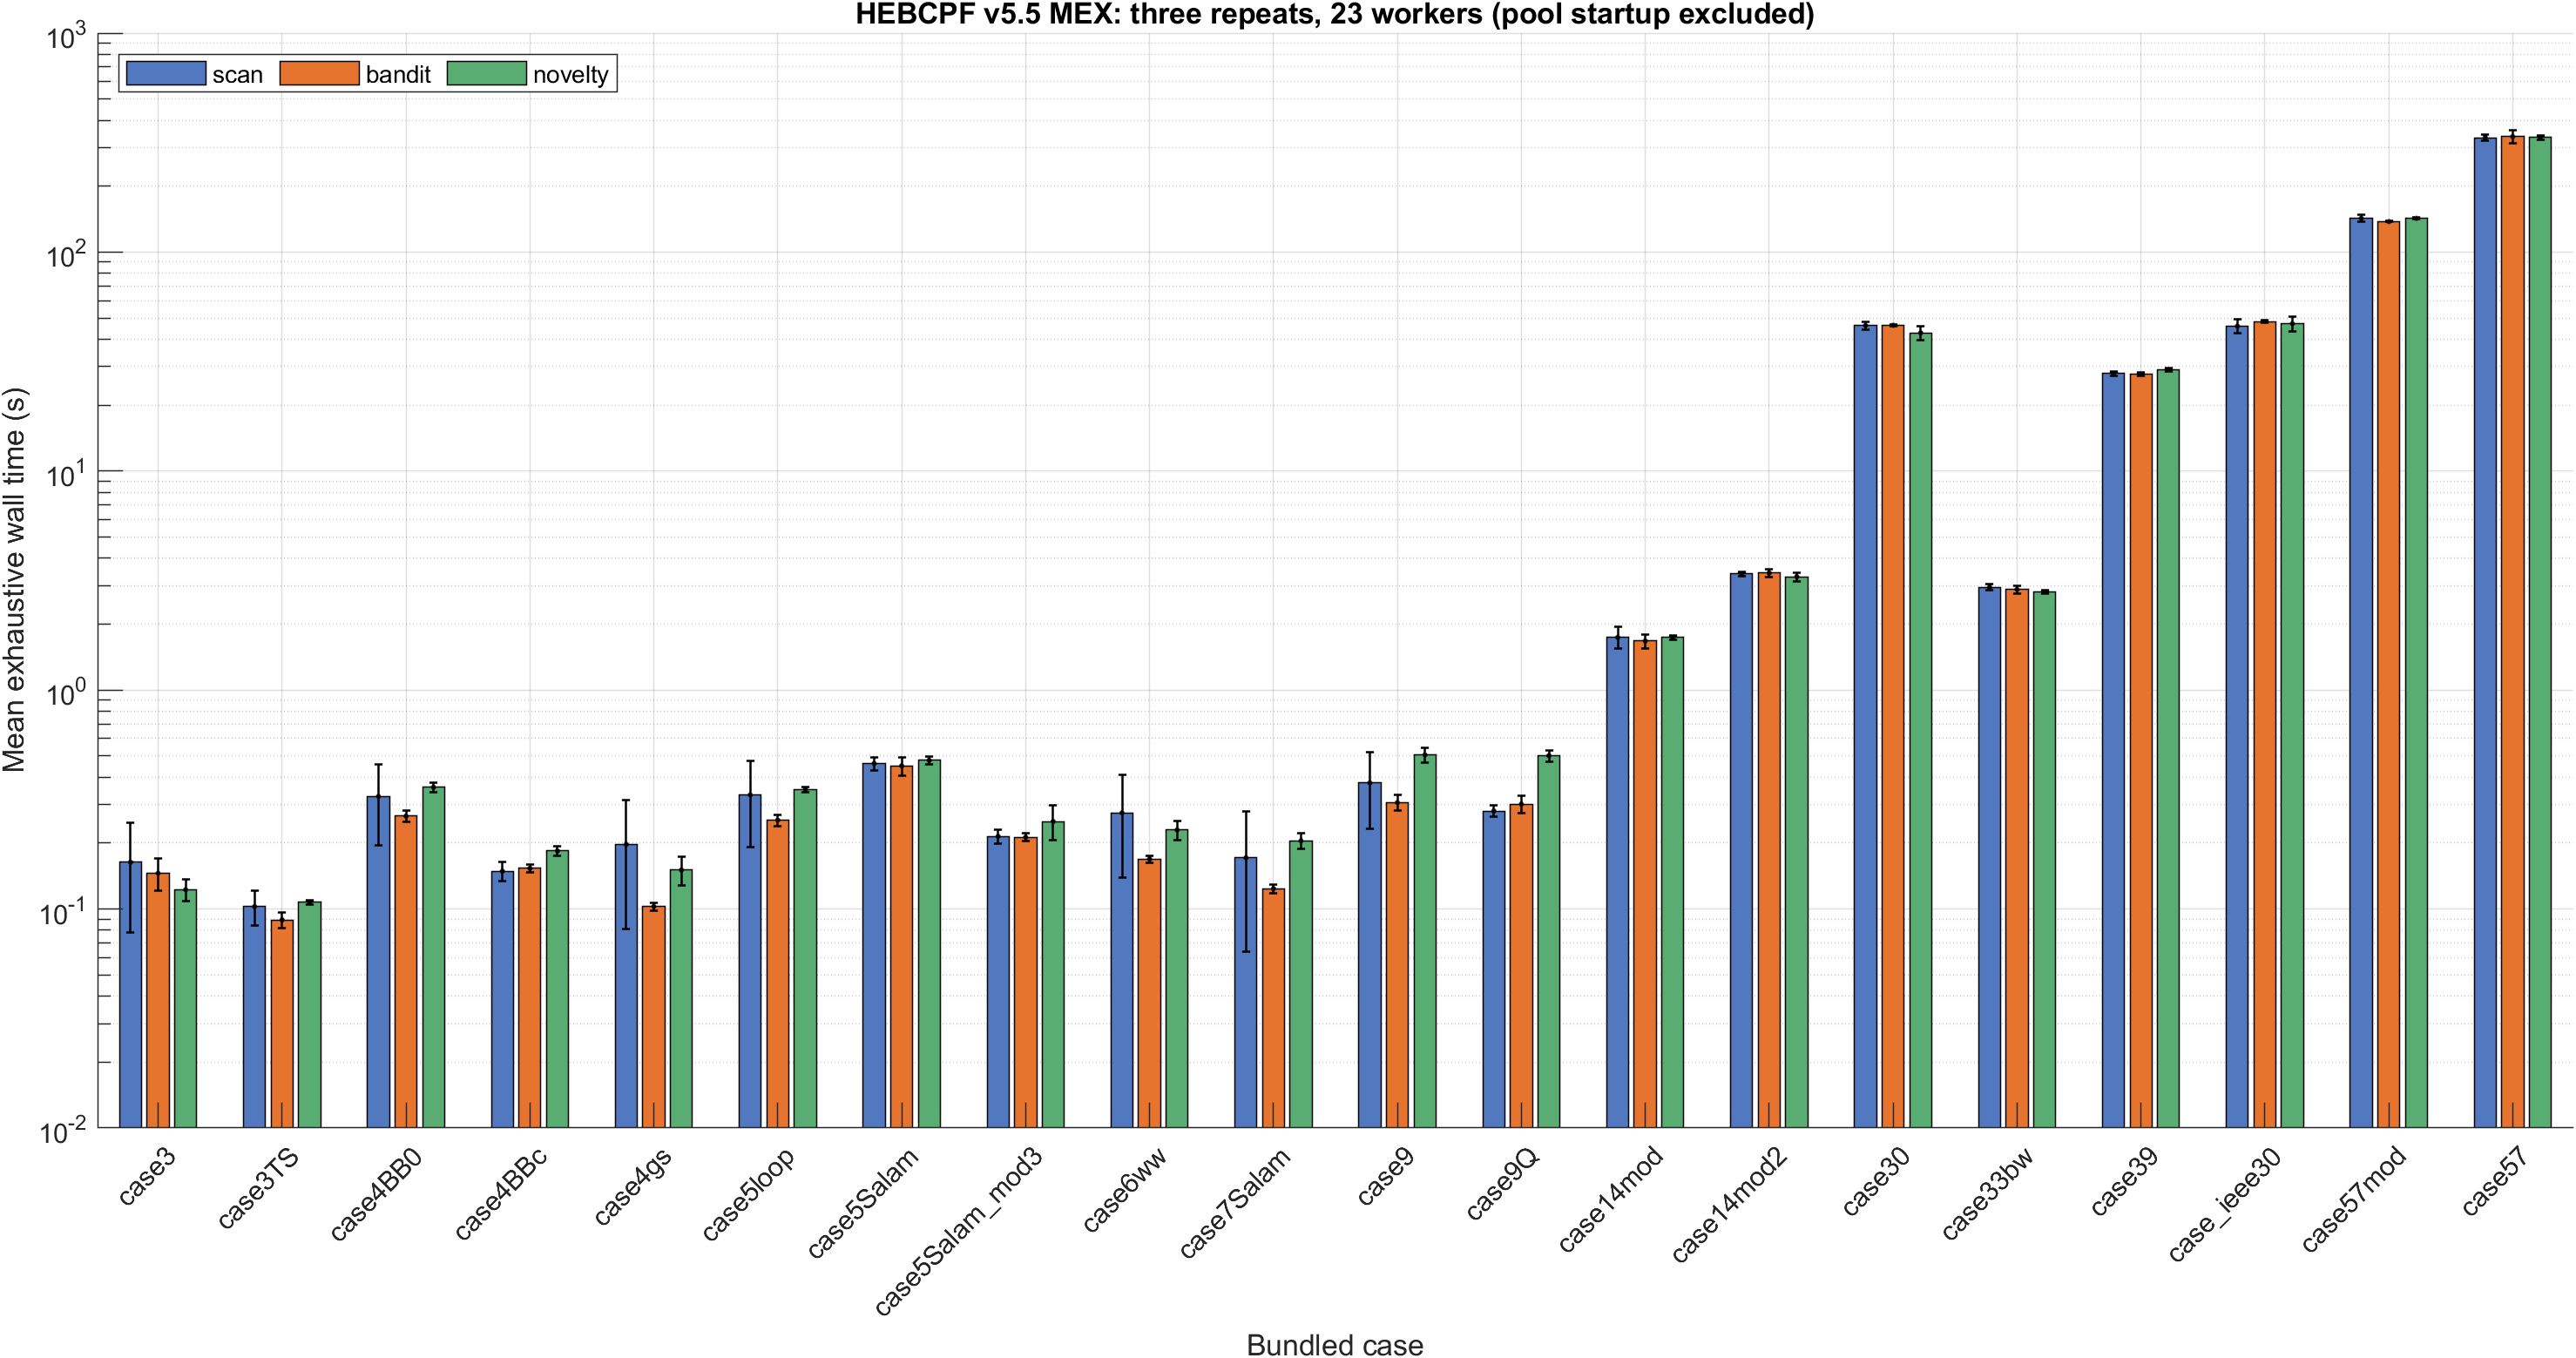
\includegraphics[width=0.96\textwidth]{scheduler_benchmark_v5_wall.png}
\caption{Three-repeat mean exhaustive MEX wall time by scheduler.}
\end{figure}}{}
\IfFileExists{scheduler_benchmark_v5_t90.png}{
\begin{figure}[htbp]\centering
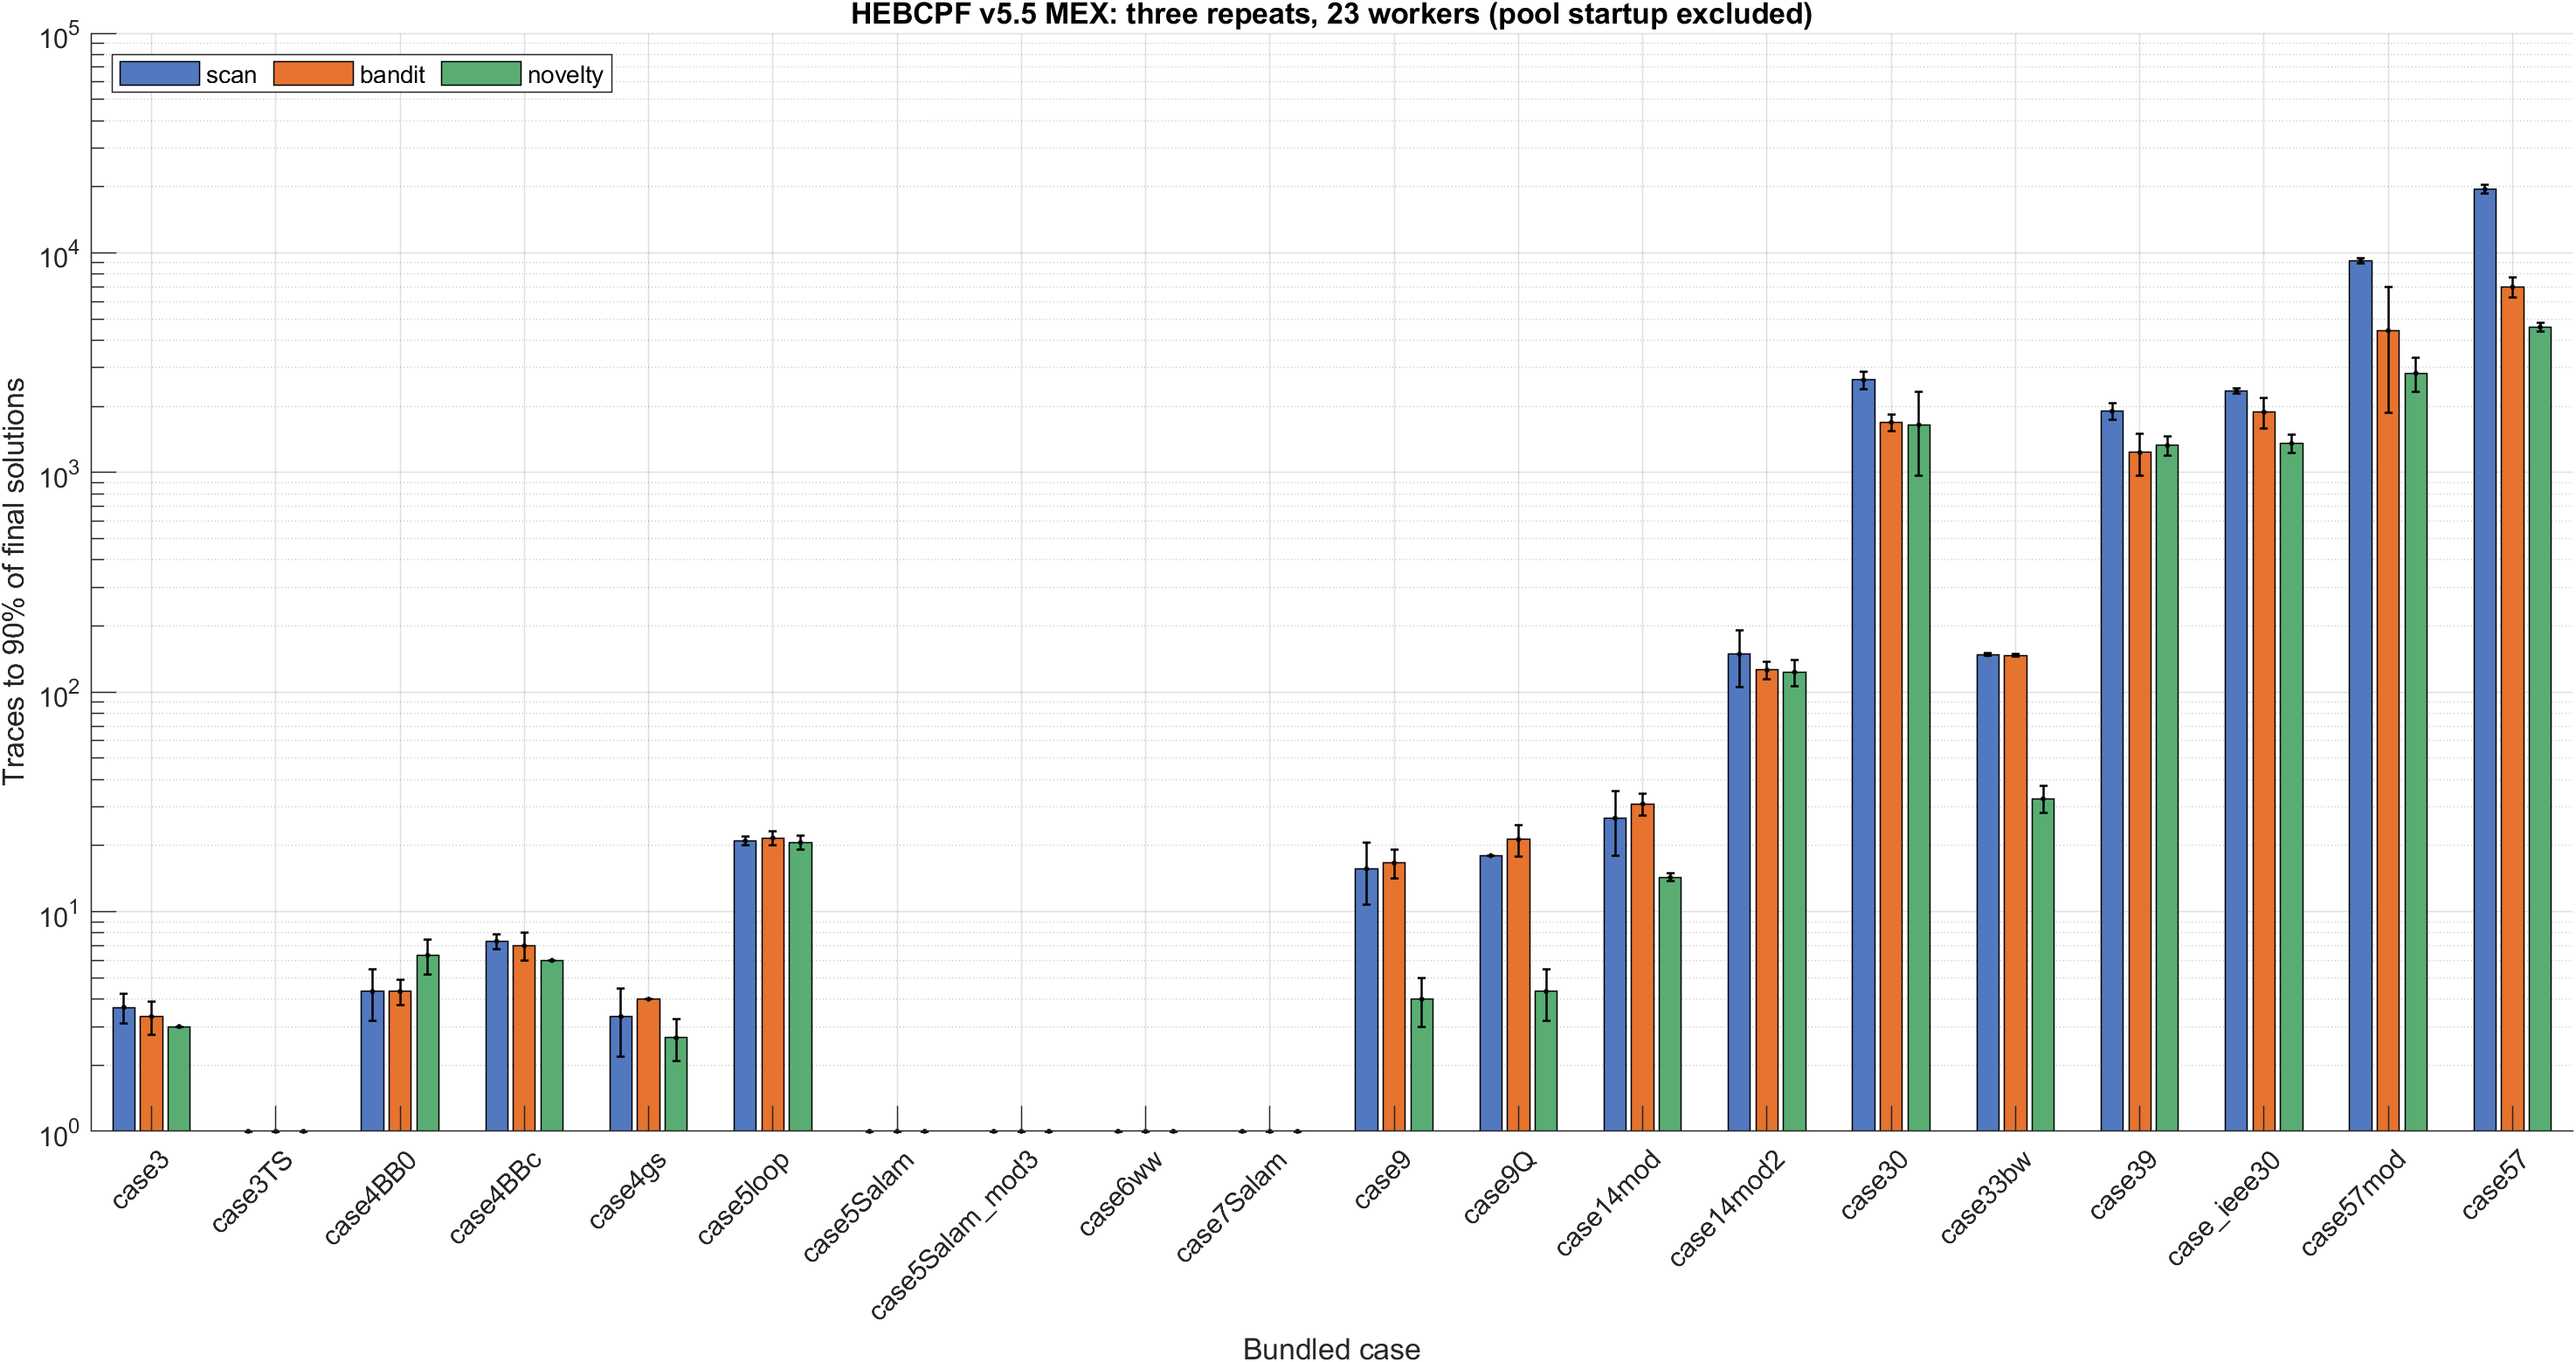
\includegraphics[width=0.96\textwidth]{scheduler_benchmark_v5_t90.png}
\caption{Mean completed traces required to reach 90\% of final solutions.}
\end{figure}}{}
\IfFileExists{scheduler_benchmark_v5_anytime.png}{
\begin{figure}[htbp]\centering
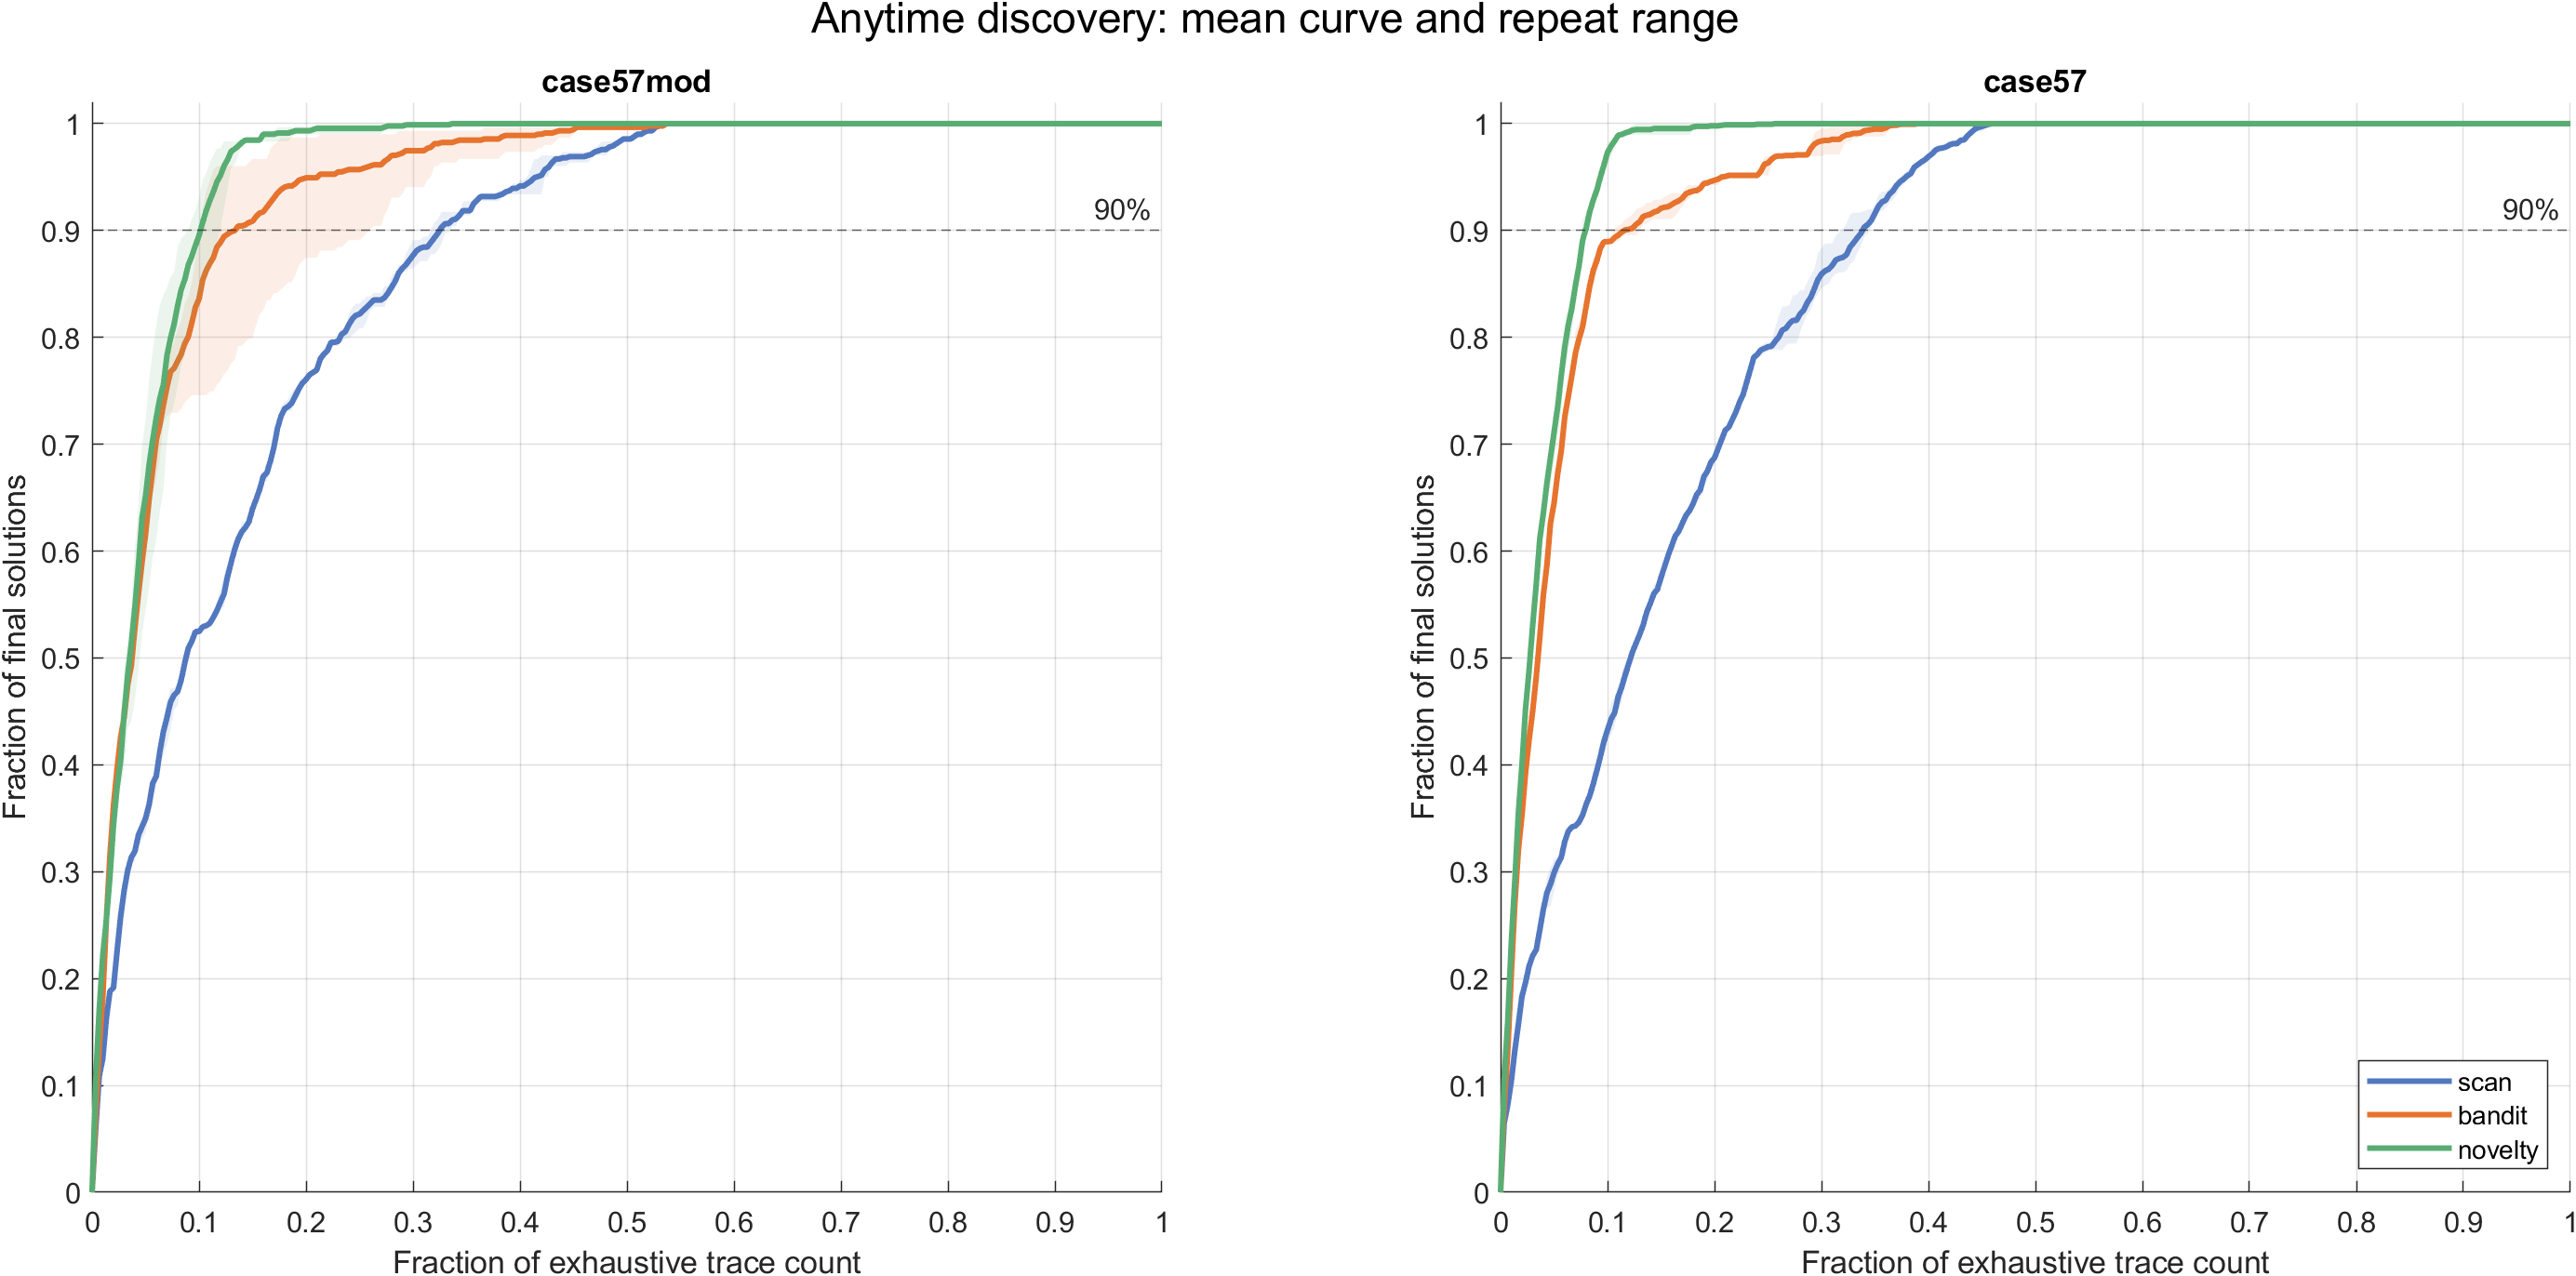
\includegraphics[width=0.96\textwidth]{scheduler_benchmark_v5_anytime.png}
\caption{Anytime discovery for case57mod and case57; bands span three repeats.}
\end{figure}}{}
\IfFileExists{scheduler_benchmark_v5_anytime_representative.png}{
\begin{figure}[htbp]\centering
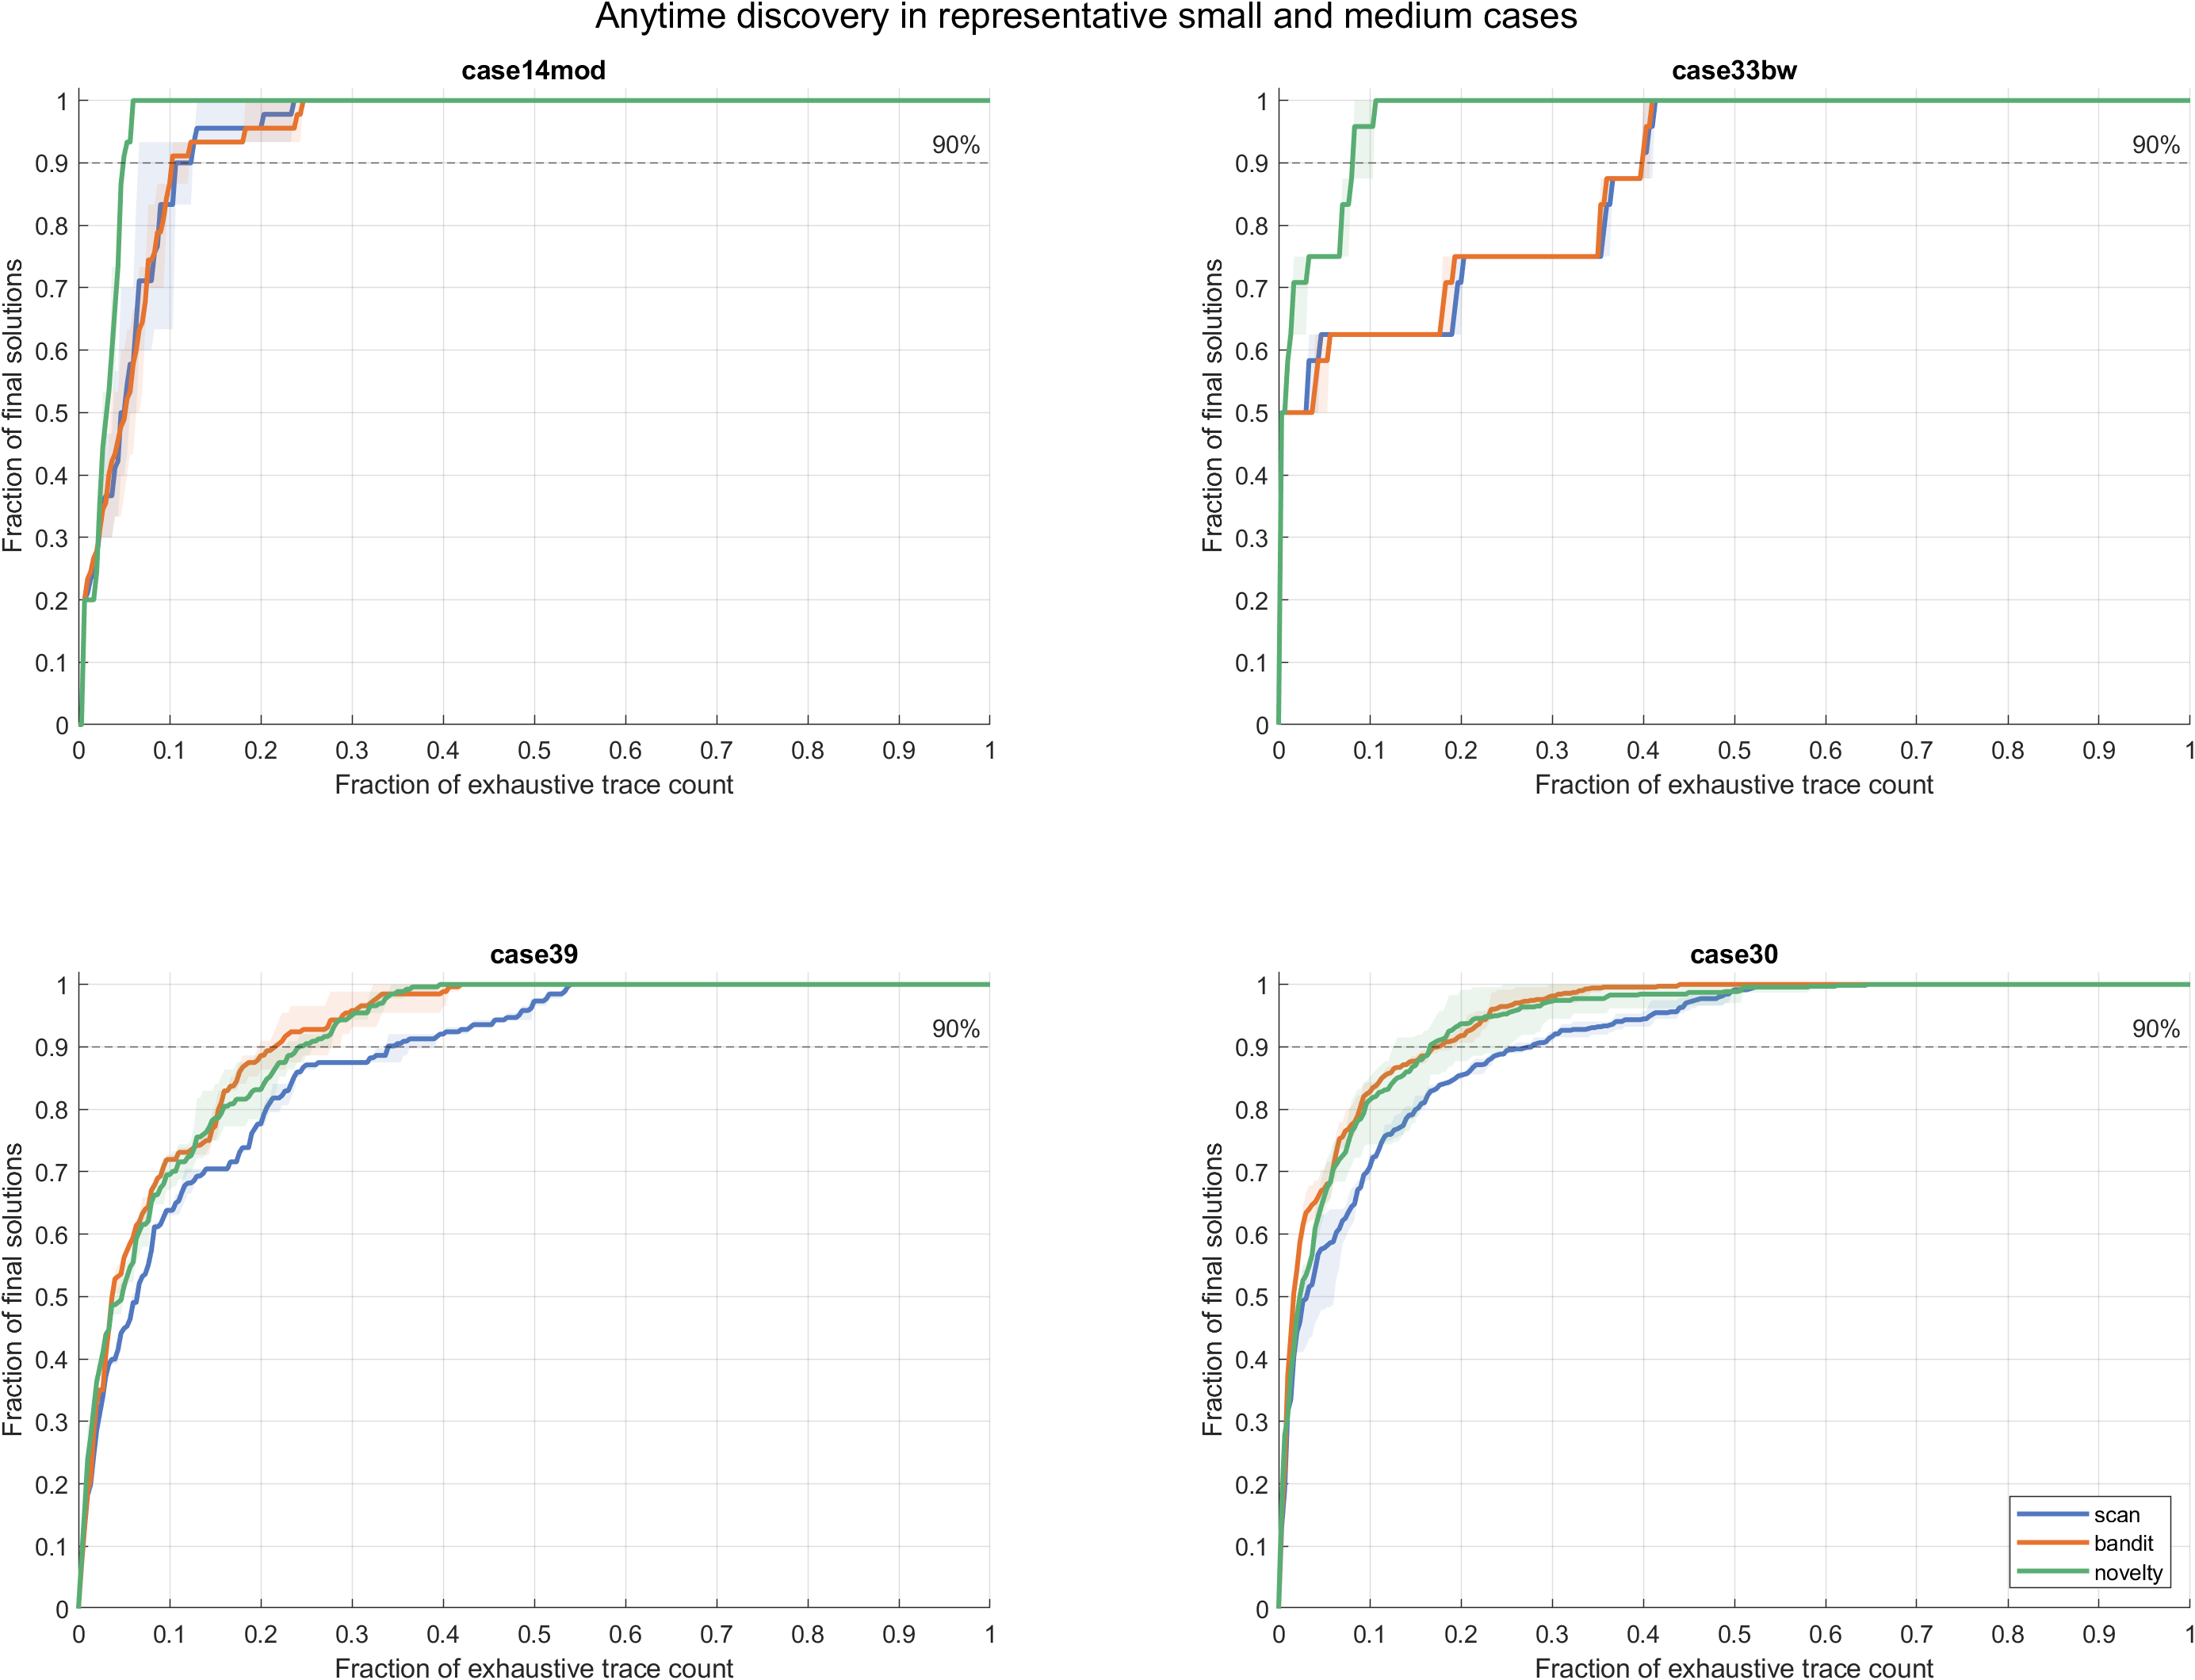
\includegraphics[width=0.96\textwidth]{scheduler_benchmark_v5_anytime_representative.png}
\caption{Recorded anytime discovery for case14mod, case33bw, case39, and case30.
Each line is the three-repeat mean and each band spans the repeat range. These
additional panels are reconstructed from saved trace histories; no solver was rerun.}
\end{figure}}{}
\IfFileExists{scheduler_benchmark_v5_anytime_suite.png}{
\begin{figure}[htbp]\centering
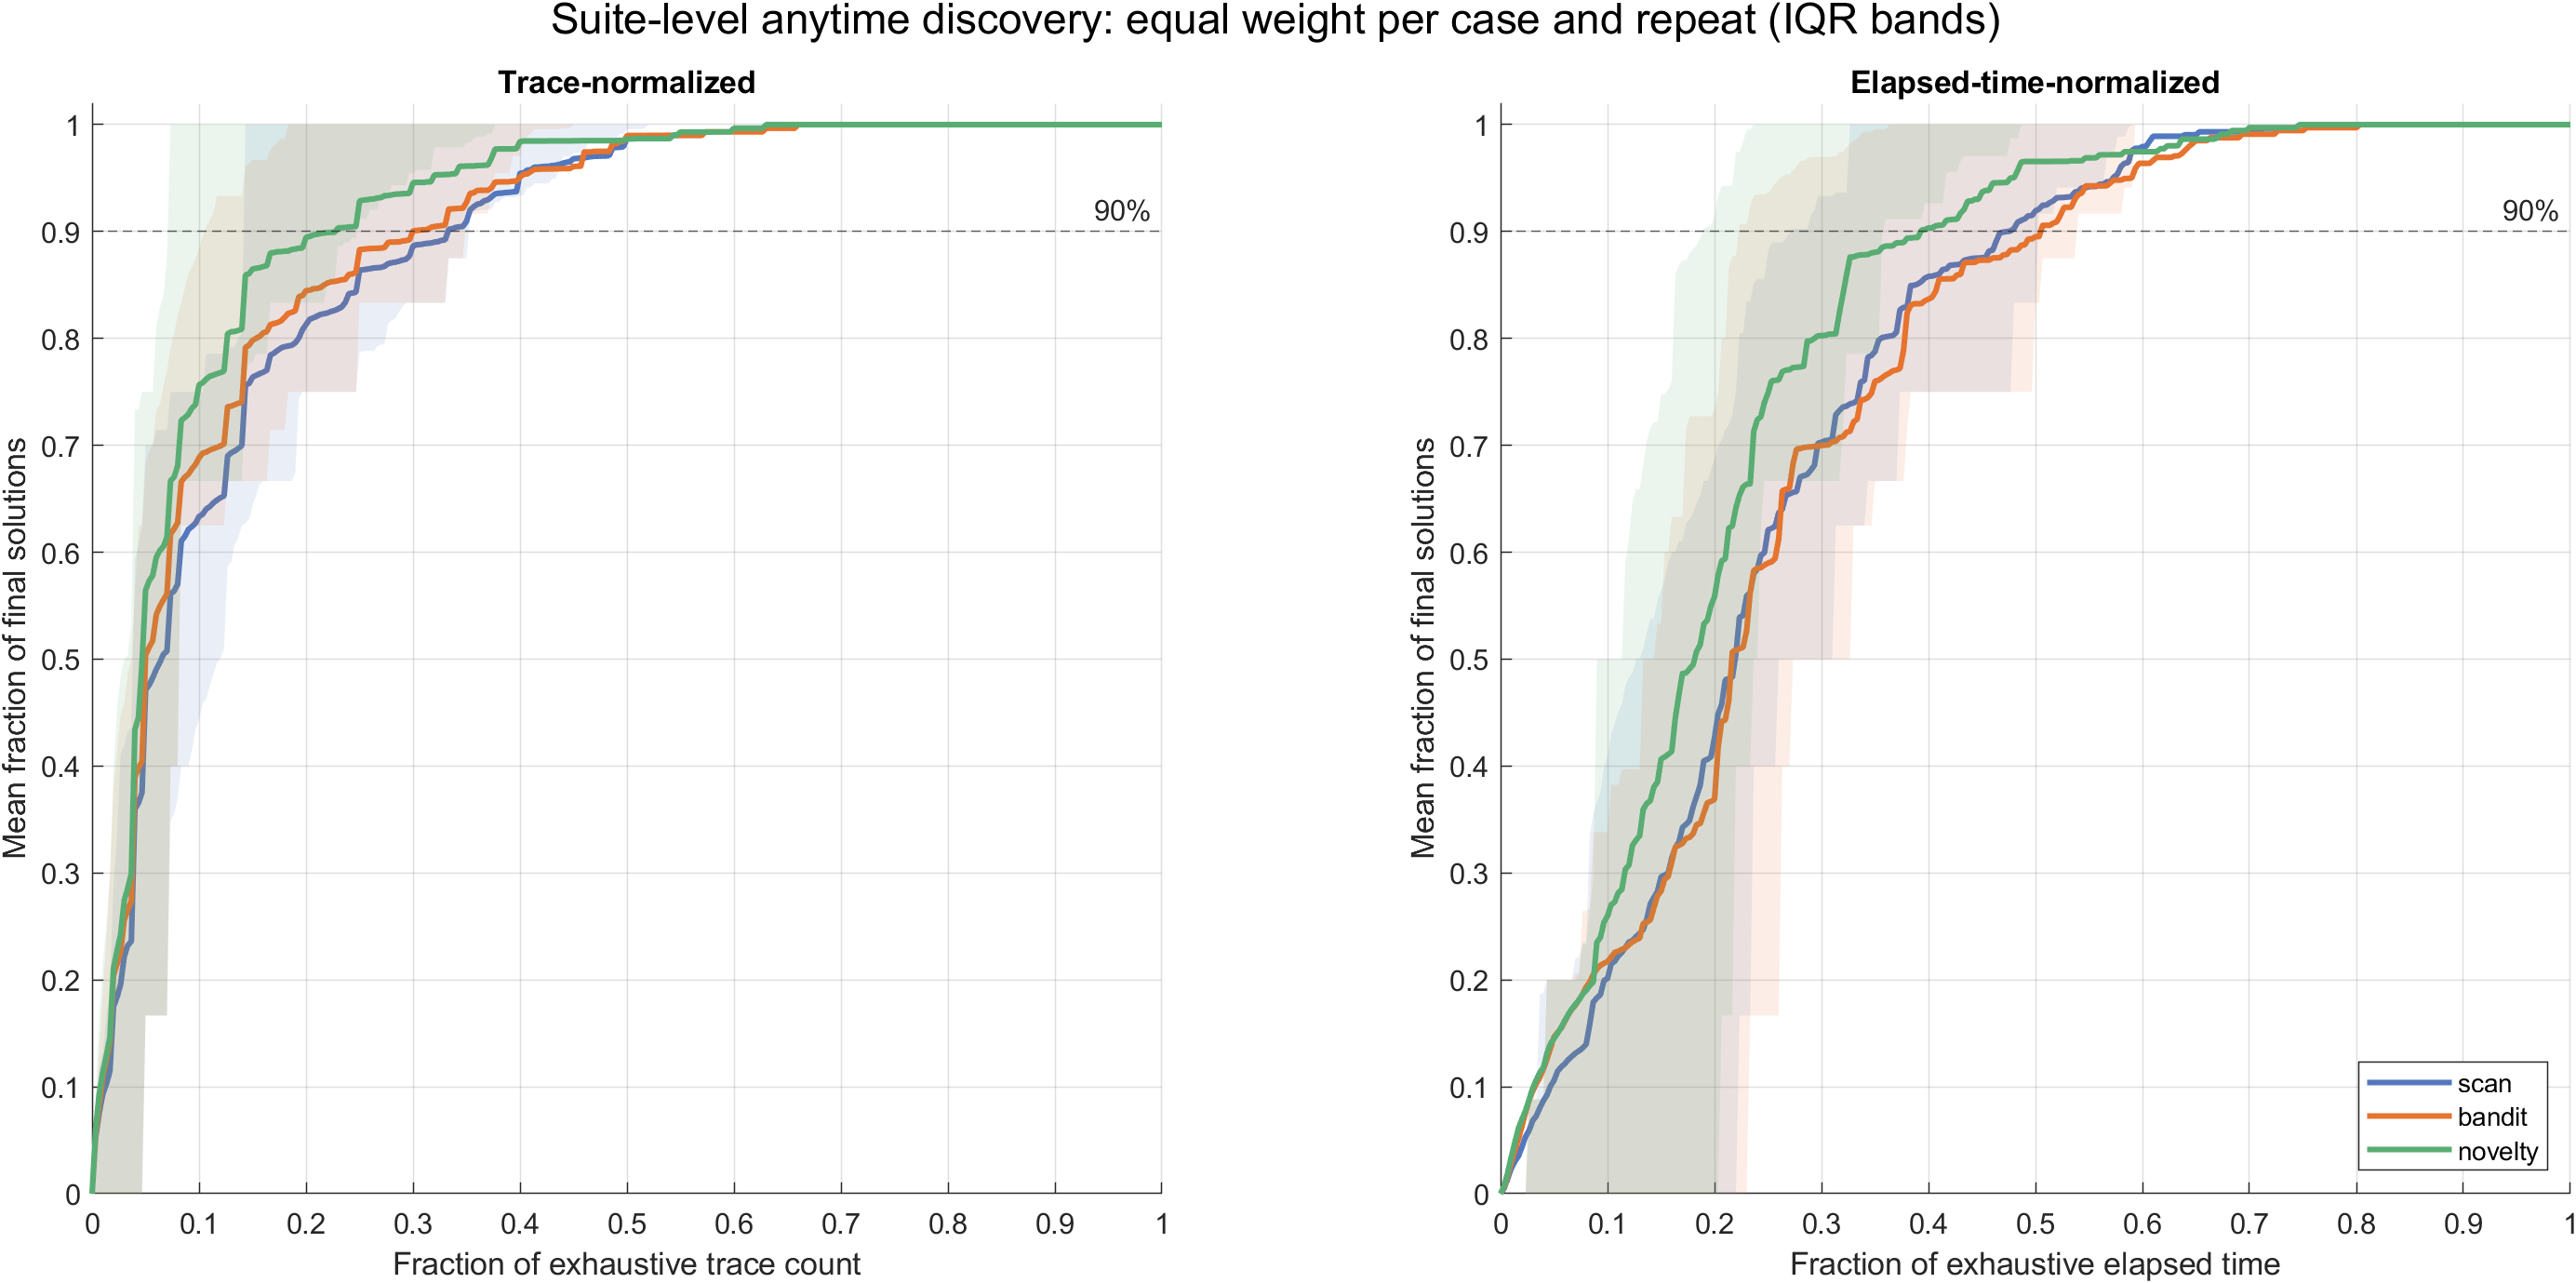
\includegraphics[width=0.96\textwidth]{scheduler_benchmark_v5_anytime_suite.png}
\caption{Suite-level normalized anytime discovery over all 20 cases. Every case
and repeat receives equal weight; bands show the interquartile range. The left
panel normalizes by exhaustive traces and the right by exhaustive elapsed time.}
\end{figure}}{}

The added case panels show that adaptive ordering is not only a case57 effect,
although the size of the advantage varies with topology and solution count. The
suite-level macro average deliberately weights every case equally, so it describes
typical normalized progress rather than allowing the two case57 variants to dominate.

The connectivity panels use one common layout per case. Nodes are accepted
solutions, color is discovery order, and edges link solutions covered by a
shared trace. Differences describe traversal history, not different final sets.

\IfFileExists{connectivity_case14mod_scan.png}{
\begin{figure}[htbp]\centering
\begin{tabular}{ccc}
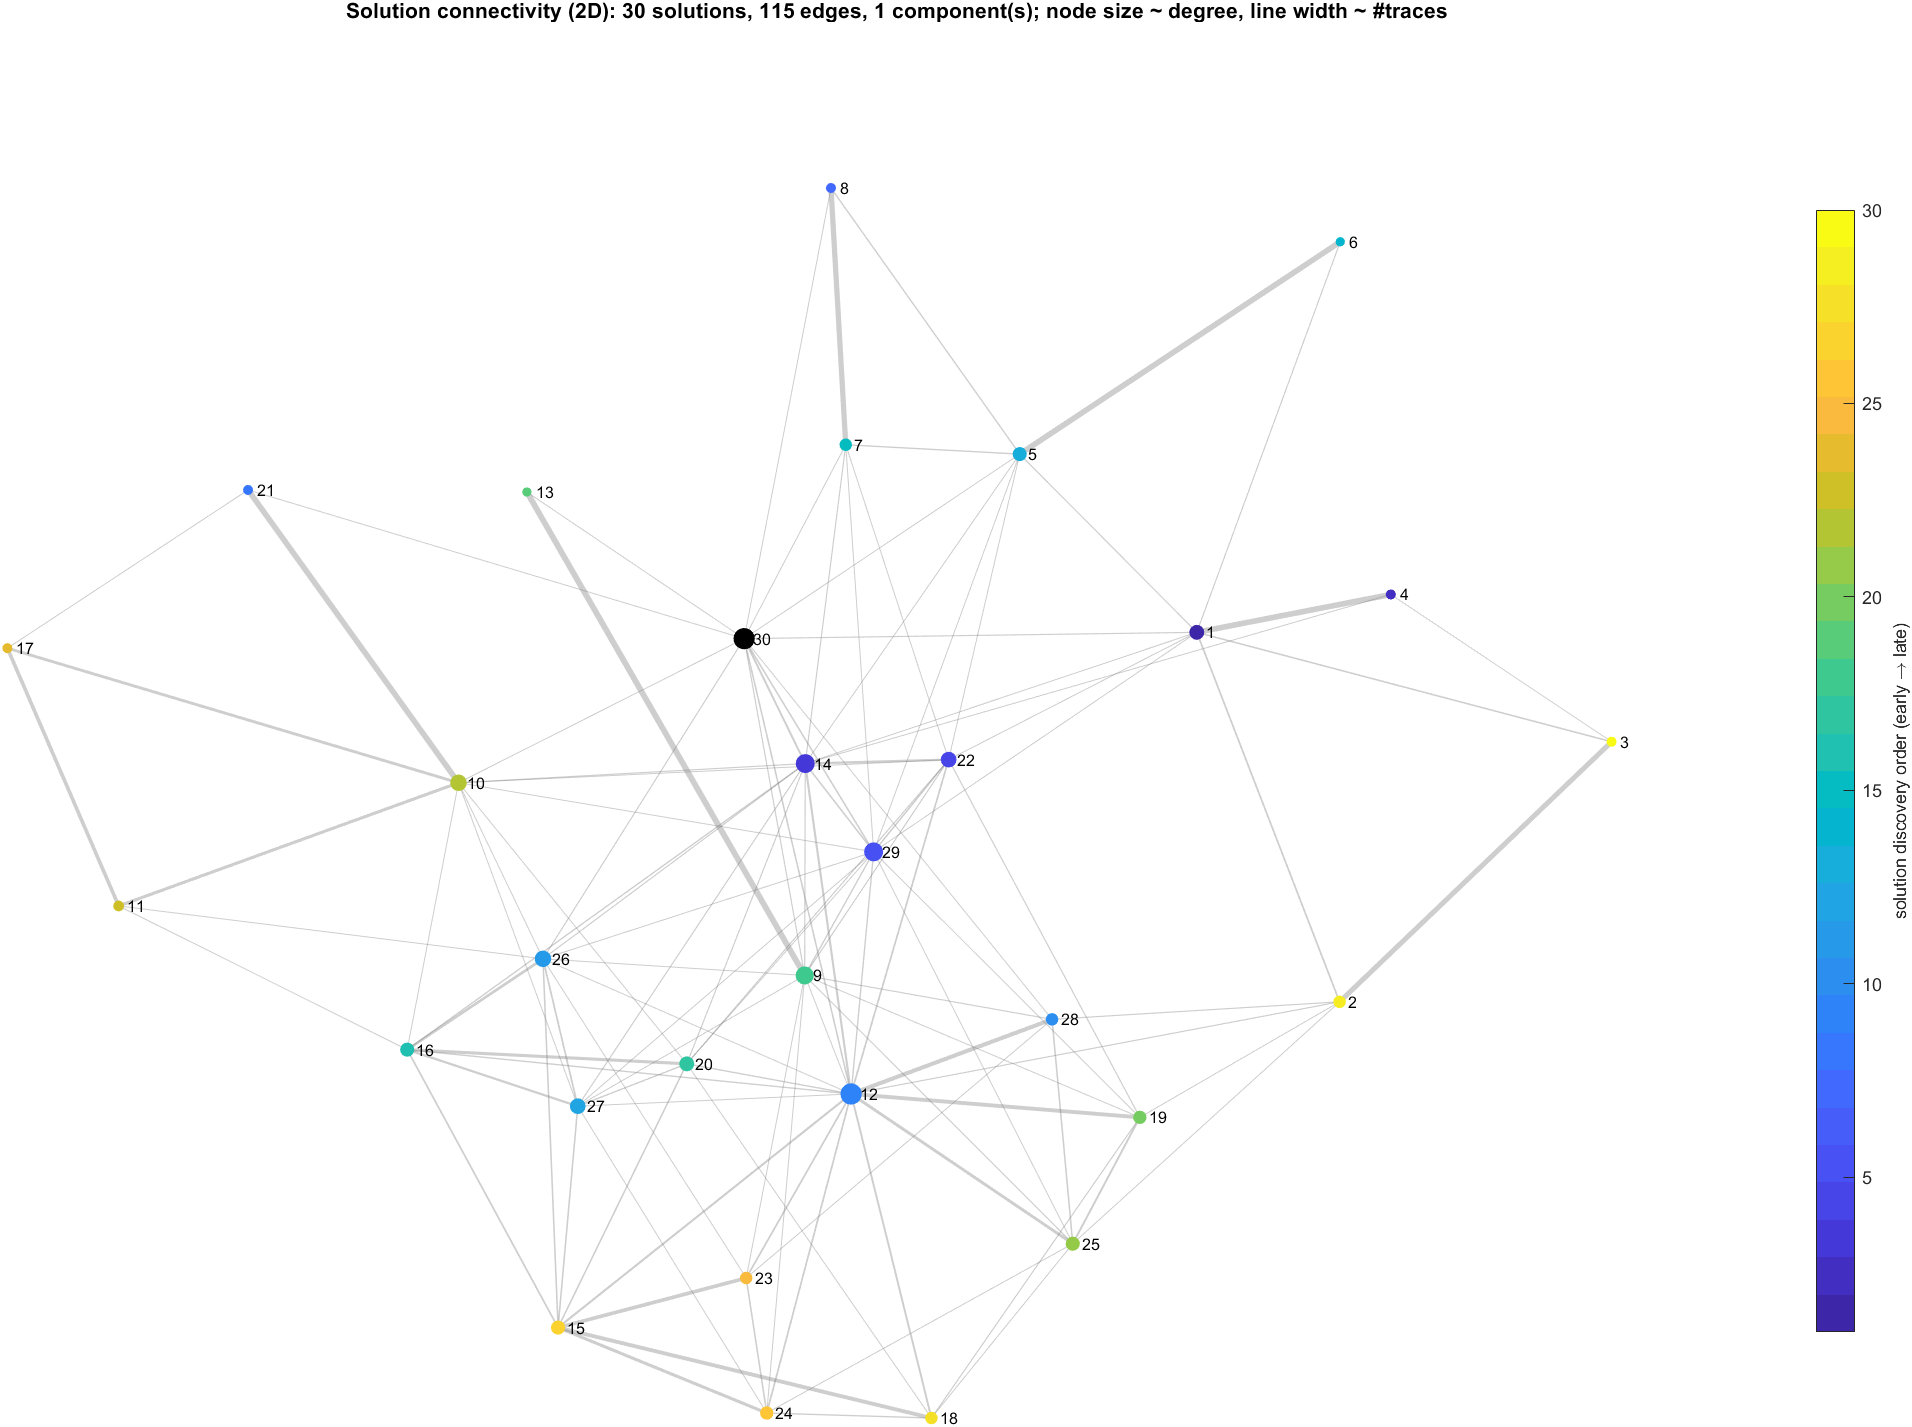
\includegraphics[width=0.30\textwidth]{connectivity_case14mod_scan.png}&
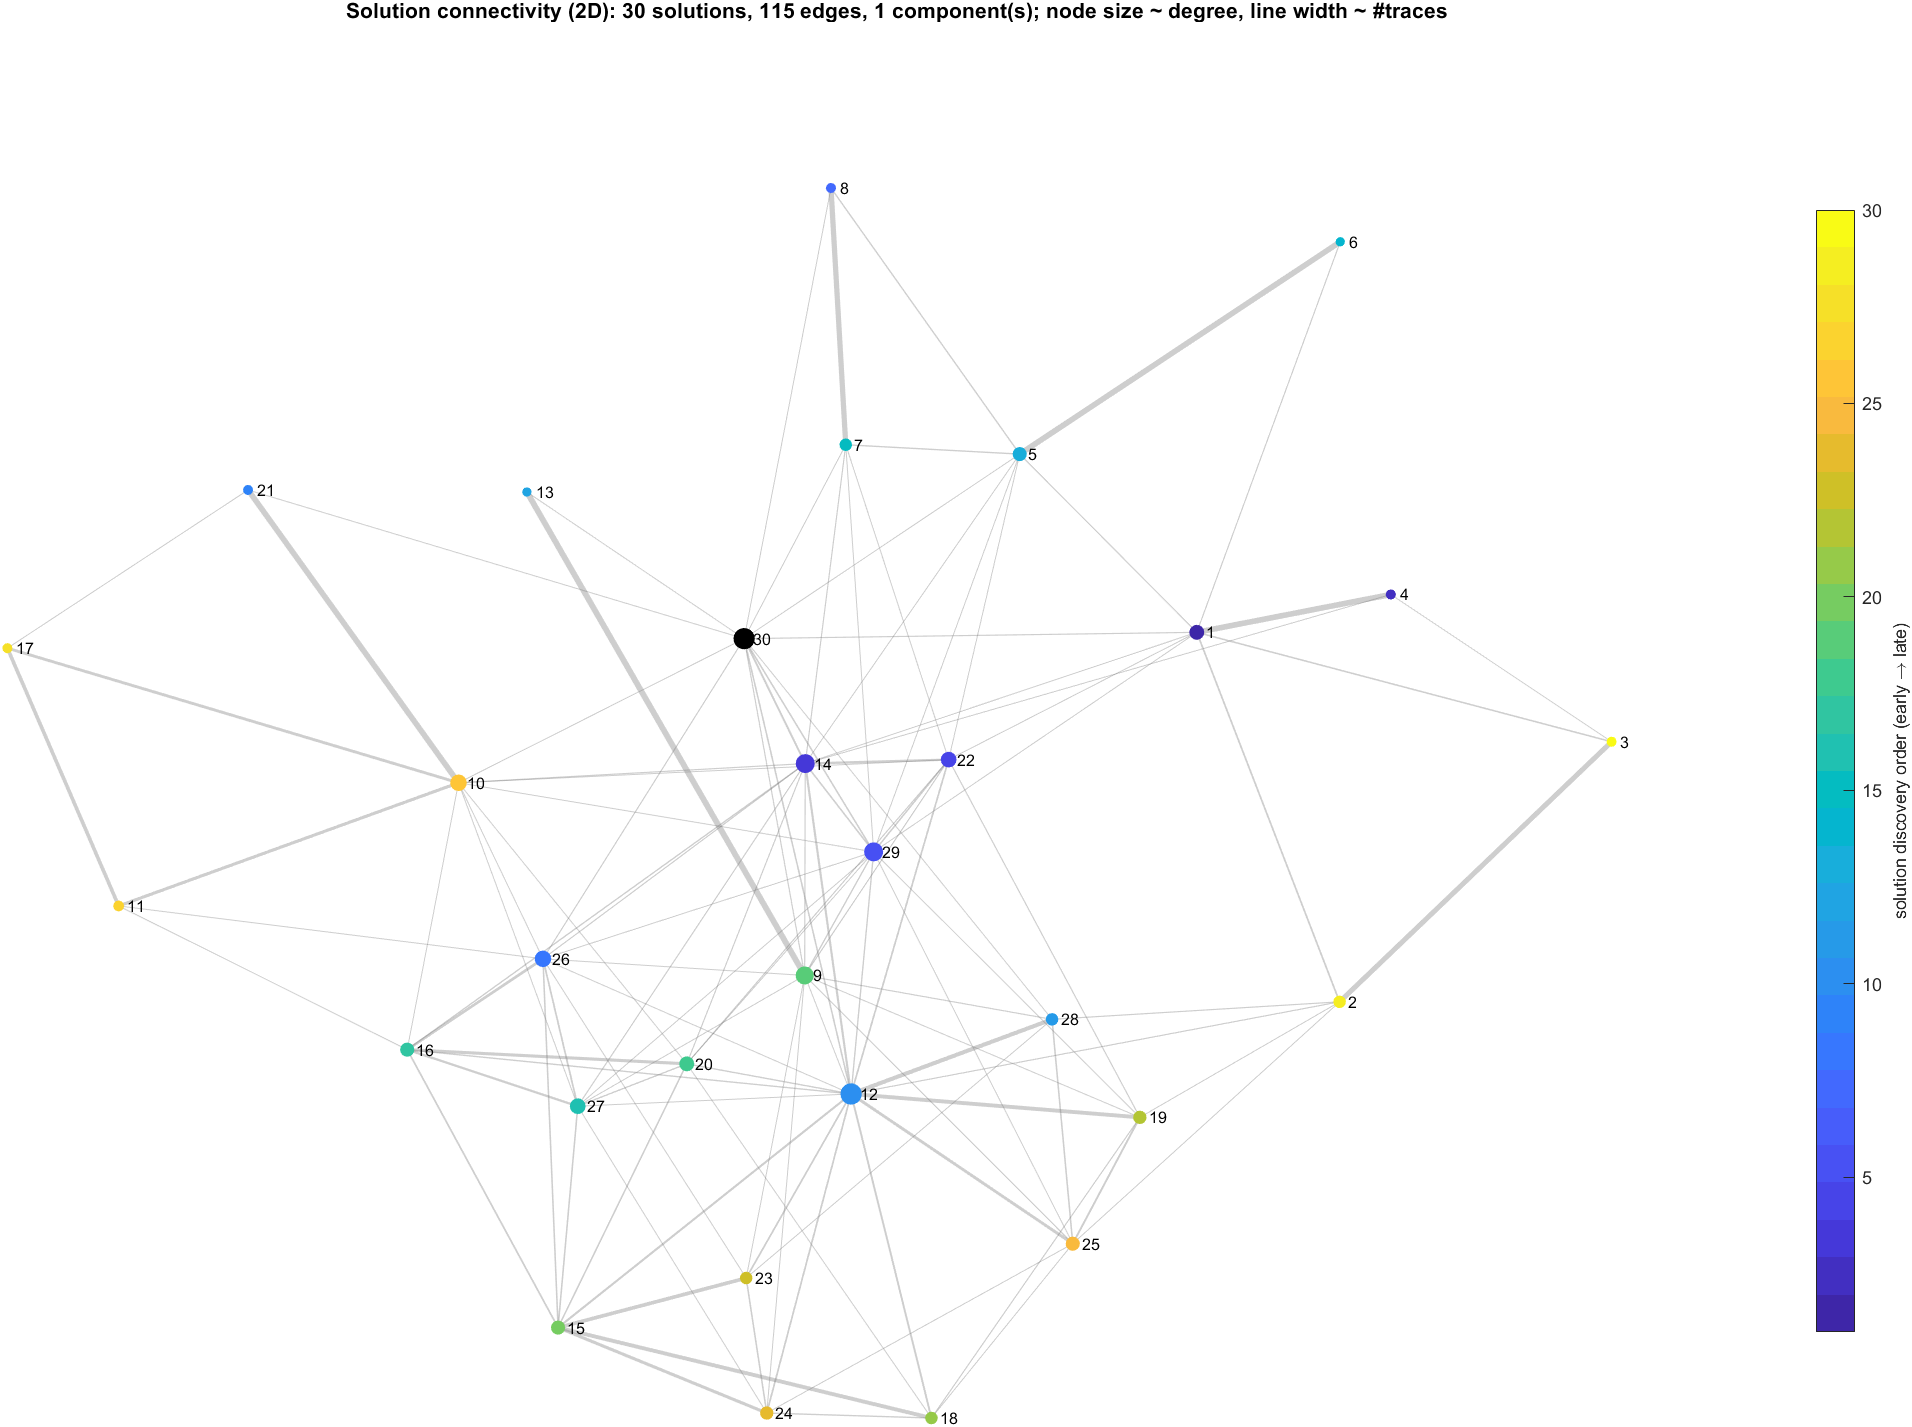
\includegraphics[width=0.30\textwidth]{connectivity_case14mod_bandit.png}&
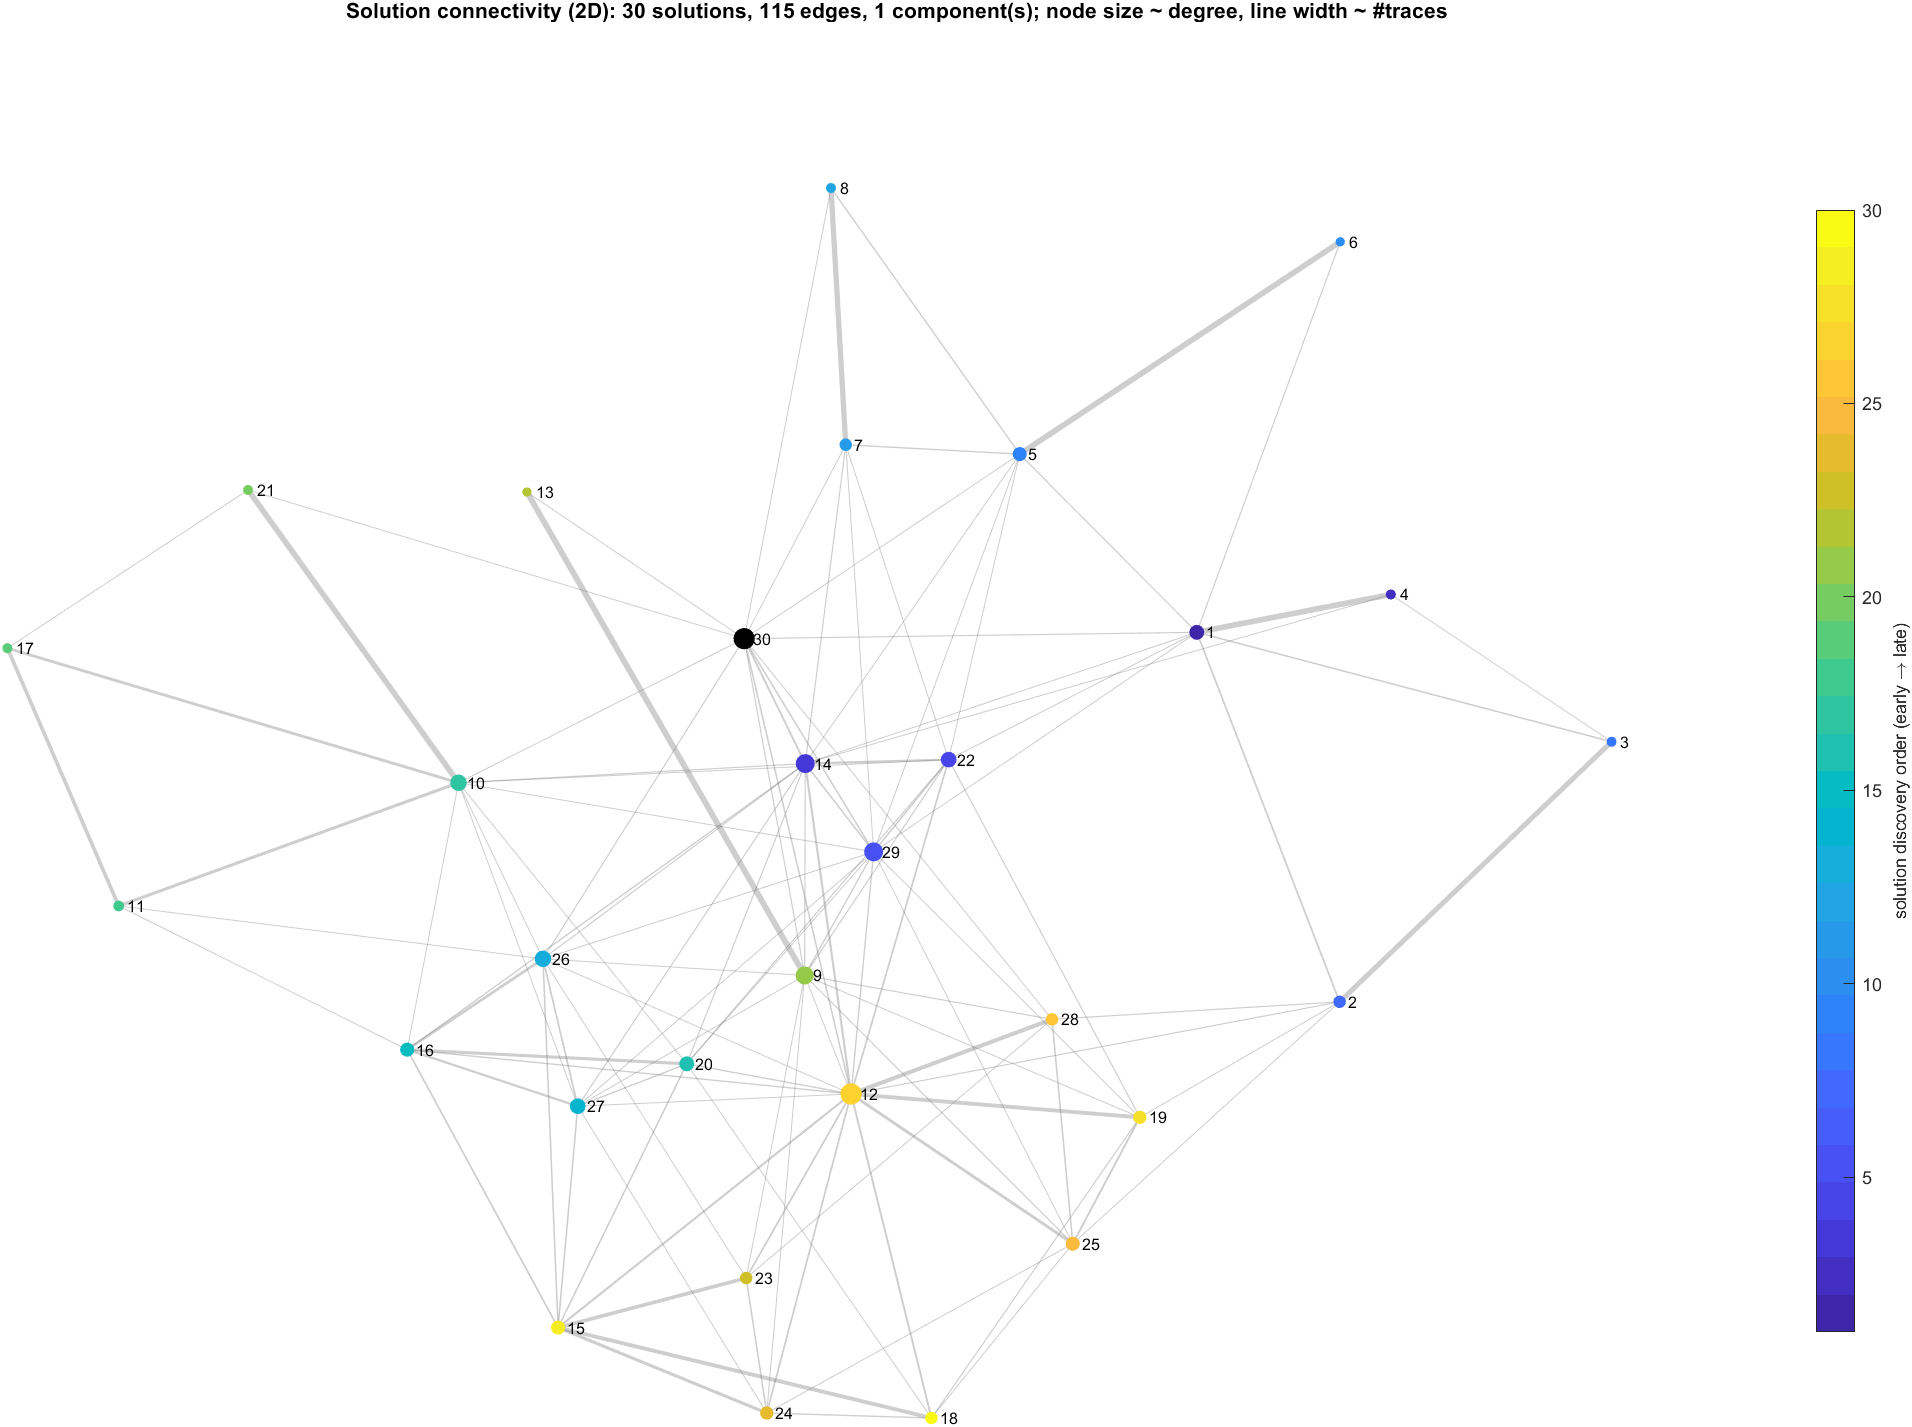
\includegraphics[width=0.30\textwidth]{connectivity_case14mod_novelty.png}\\
\code{scan}&\code{bandit}&\code{novelty}
\end{tabular}
\caption{case14mod connectivity for the common 30-solution set.}
\end{figure}}{}
\IfFileExists{connectivity_case39_scan.png}{
\begin{figure}[htbp]\centering
\begin{tabular}{ccc}
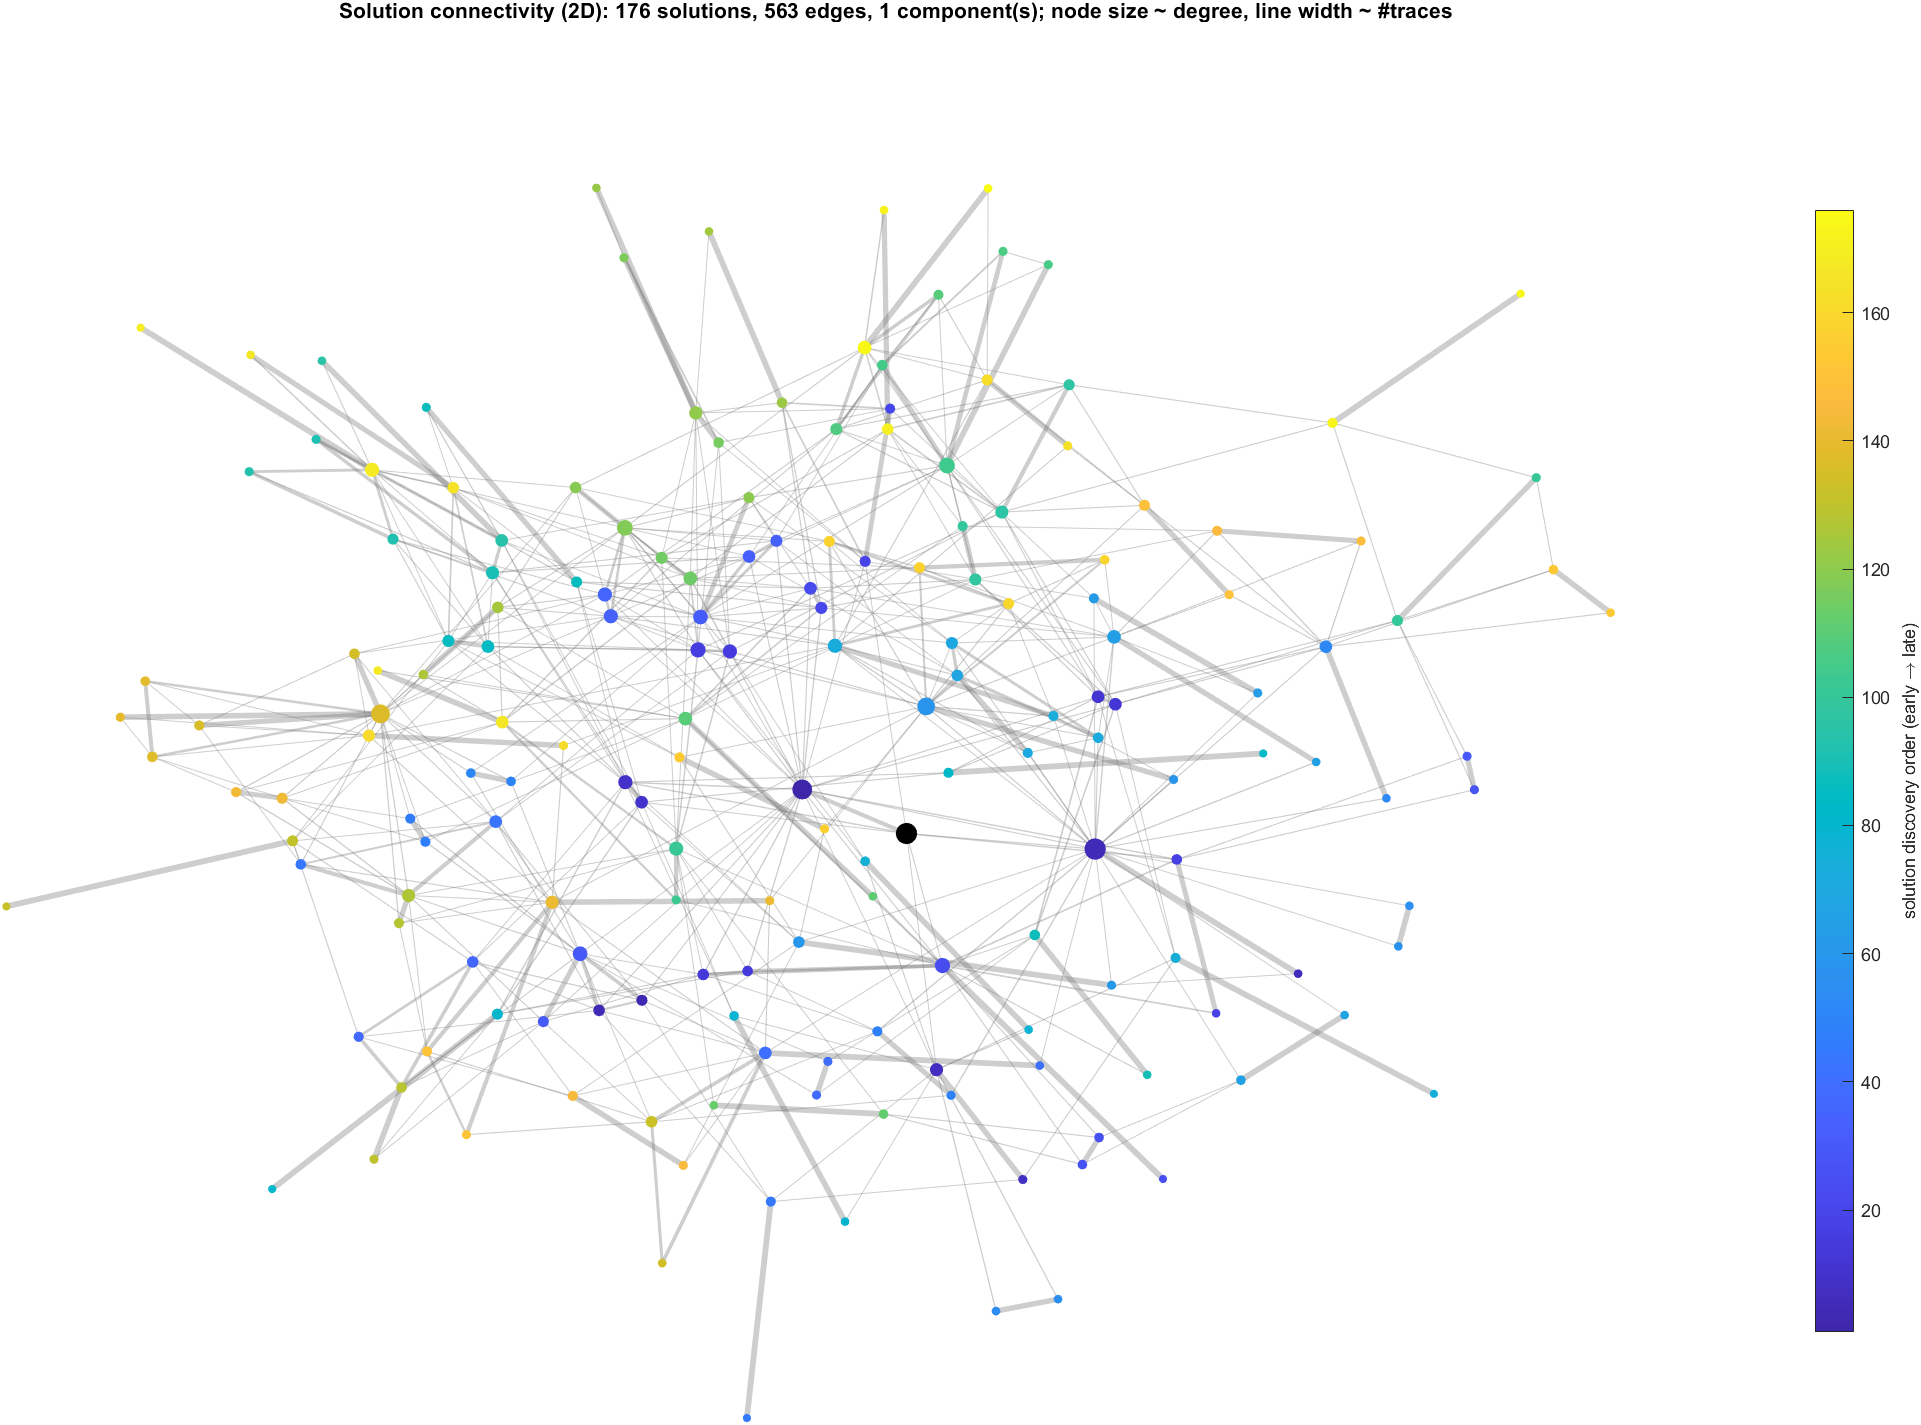
\includegraphics[width=0.30\textwidth]{connectivity_case39_scan.png}&
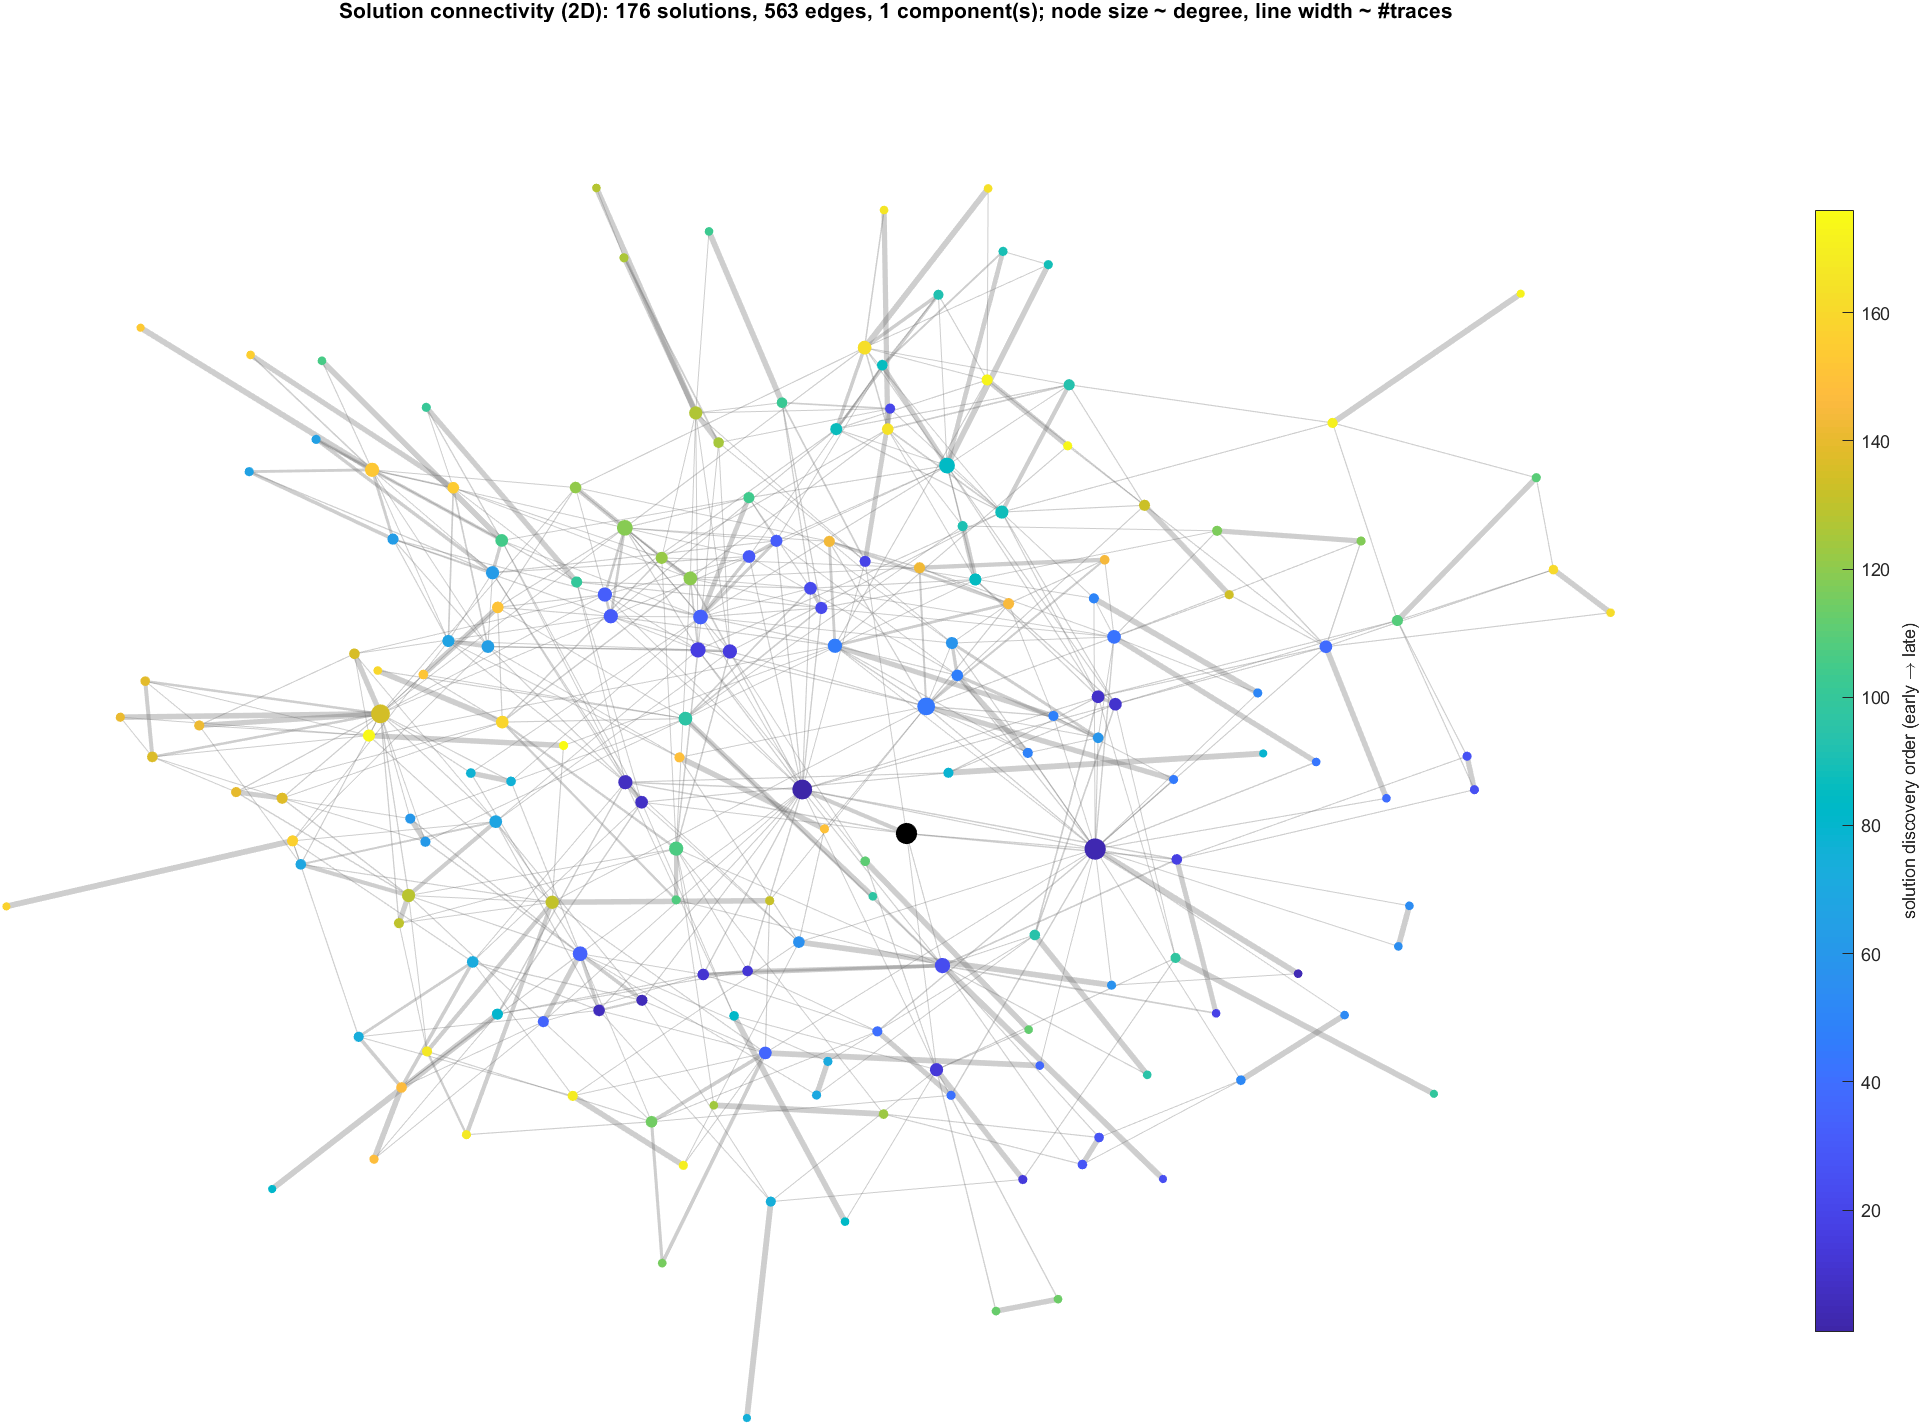
\includegraphics[width=0.30\textwidth]{connectivity_case39_bandit.png}&
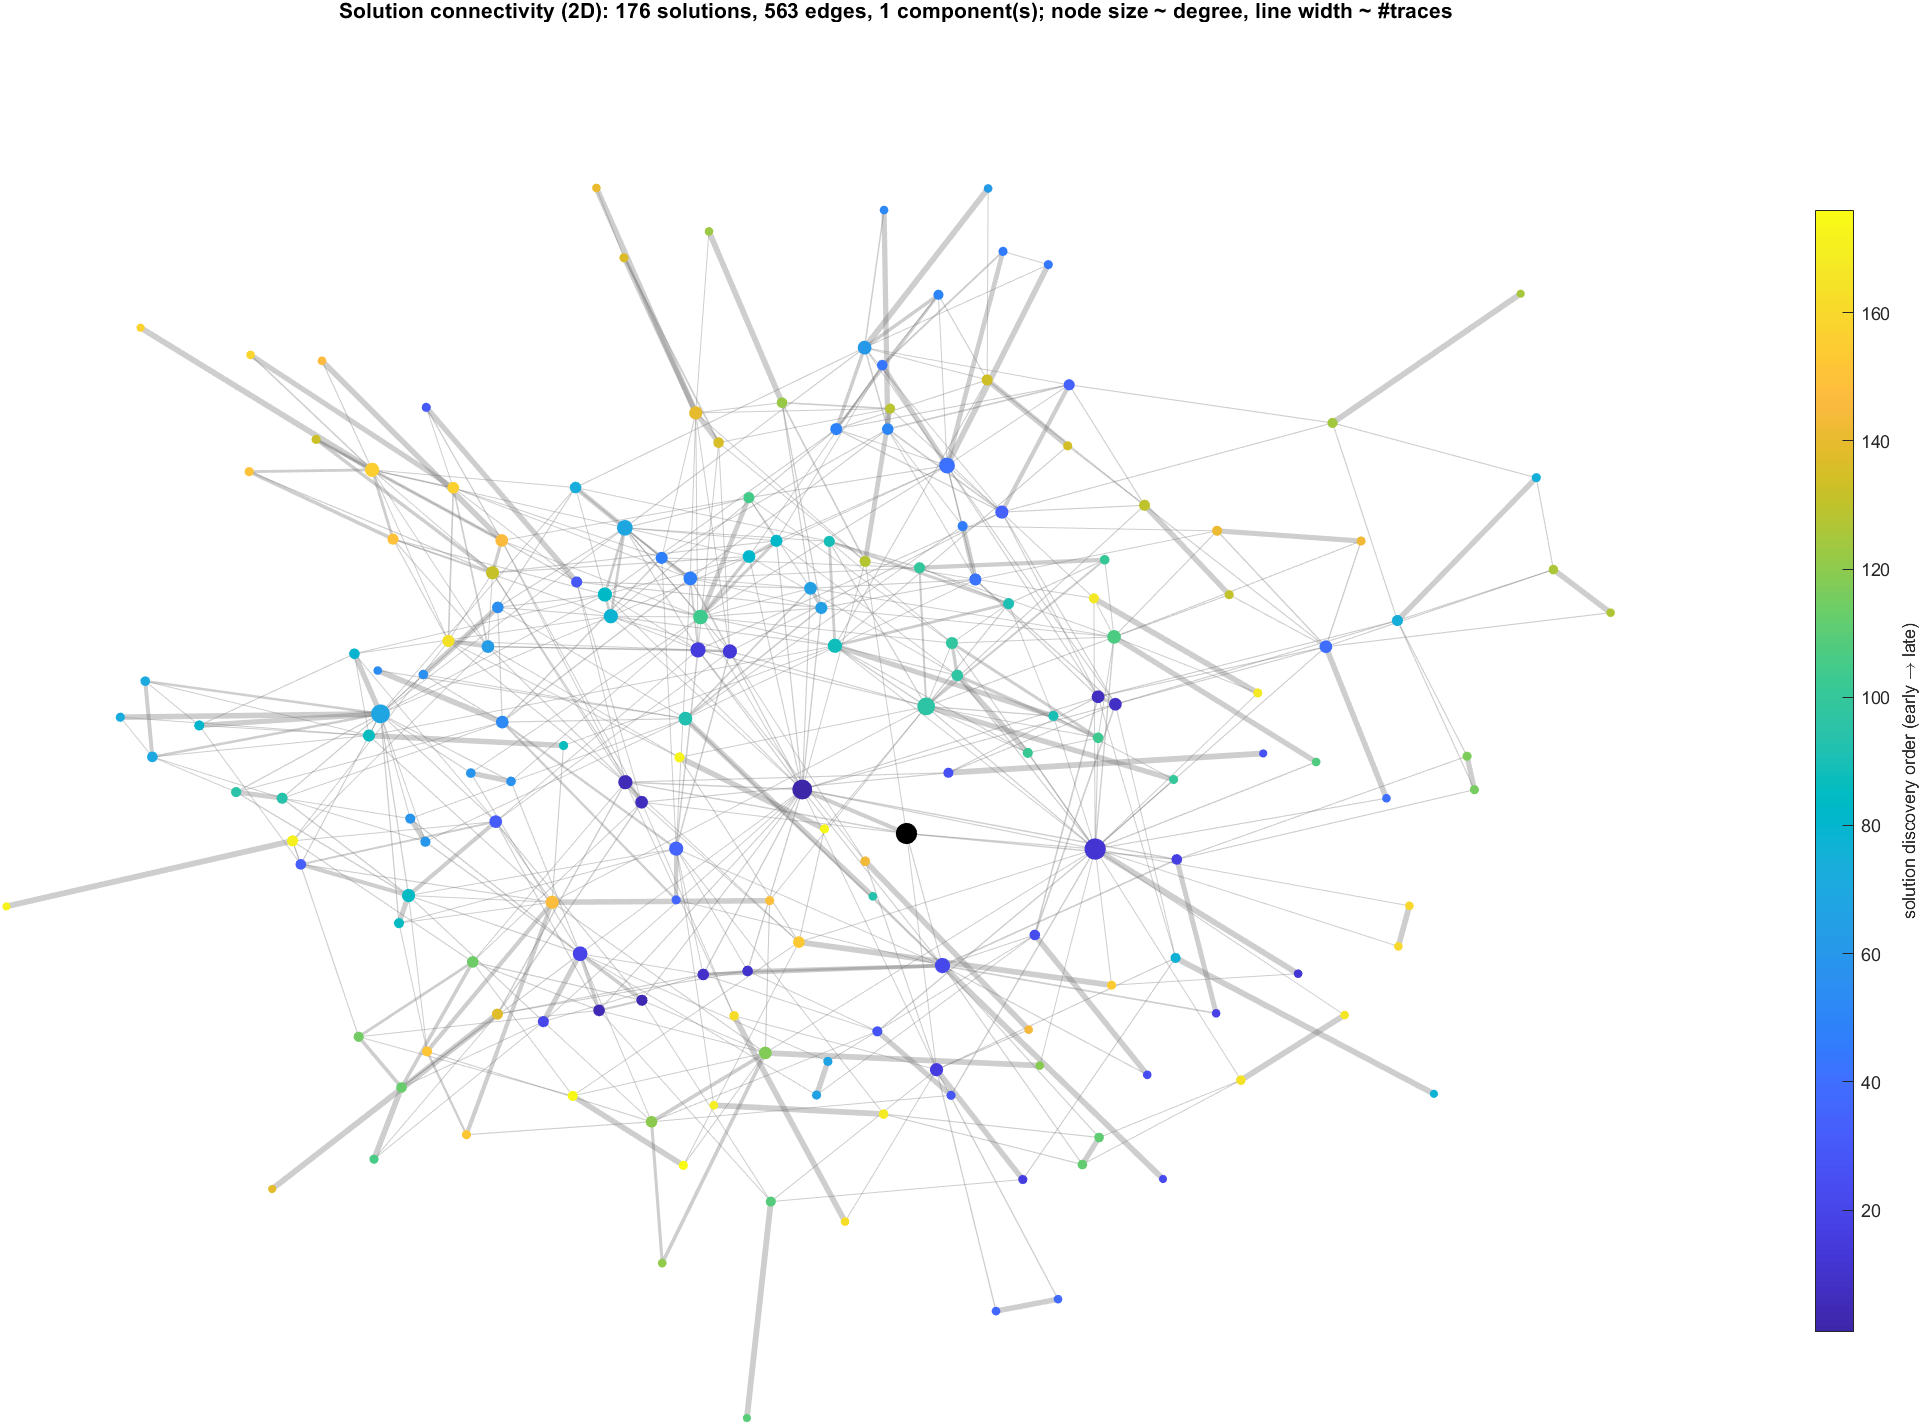
\includegraphics[width=0.30\textwidth]{connectivity_case39_novelty.png}\\
\code{scan}&\code{bandit}&\code{novelty}
\end{tabular}
\caption{case39 connectivity for the validated common 176-solution set.}
\end{figure}}{}

The scheduler benchmark retained final solution matrices and cumulative
per-trace discovery histories for case30 and case57, but it did not retain the
large policy-specific \code{VBook} arrays needed to reconstruct exact
scan/bandit/novelty edges. The following two figures are therefore explicitly
reference traversal graphs reconstructed offline from the complete released-v4
MEX snapshots. Their saved solution matrices agree with the v5 scan references
well inside the $4\times10^{-7}$ tolerance; they must not be interpreted as
three-policy v5 traversal comparisons.

\IfFileExists{connectivity_case30_v4_reference.png}{
\begin{figure}[p]\centering
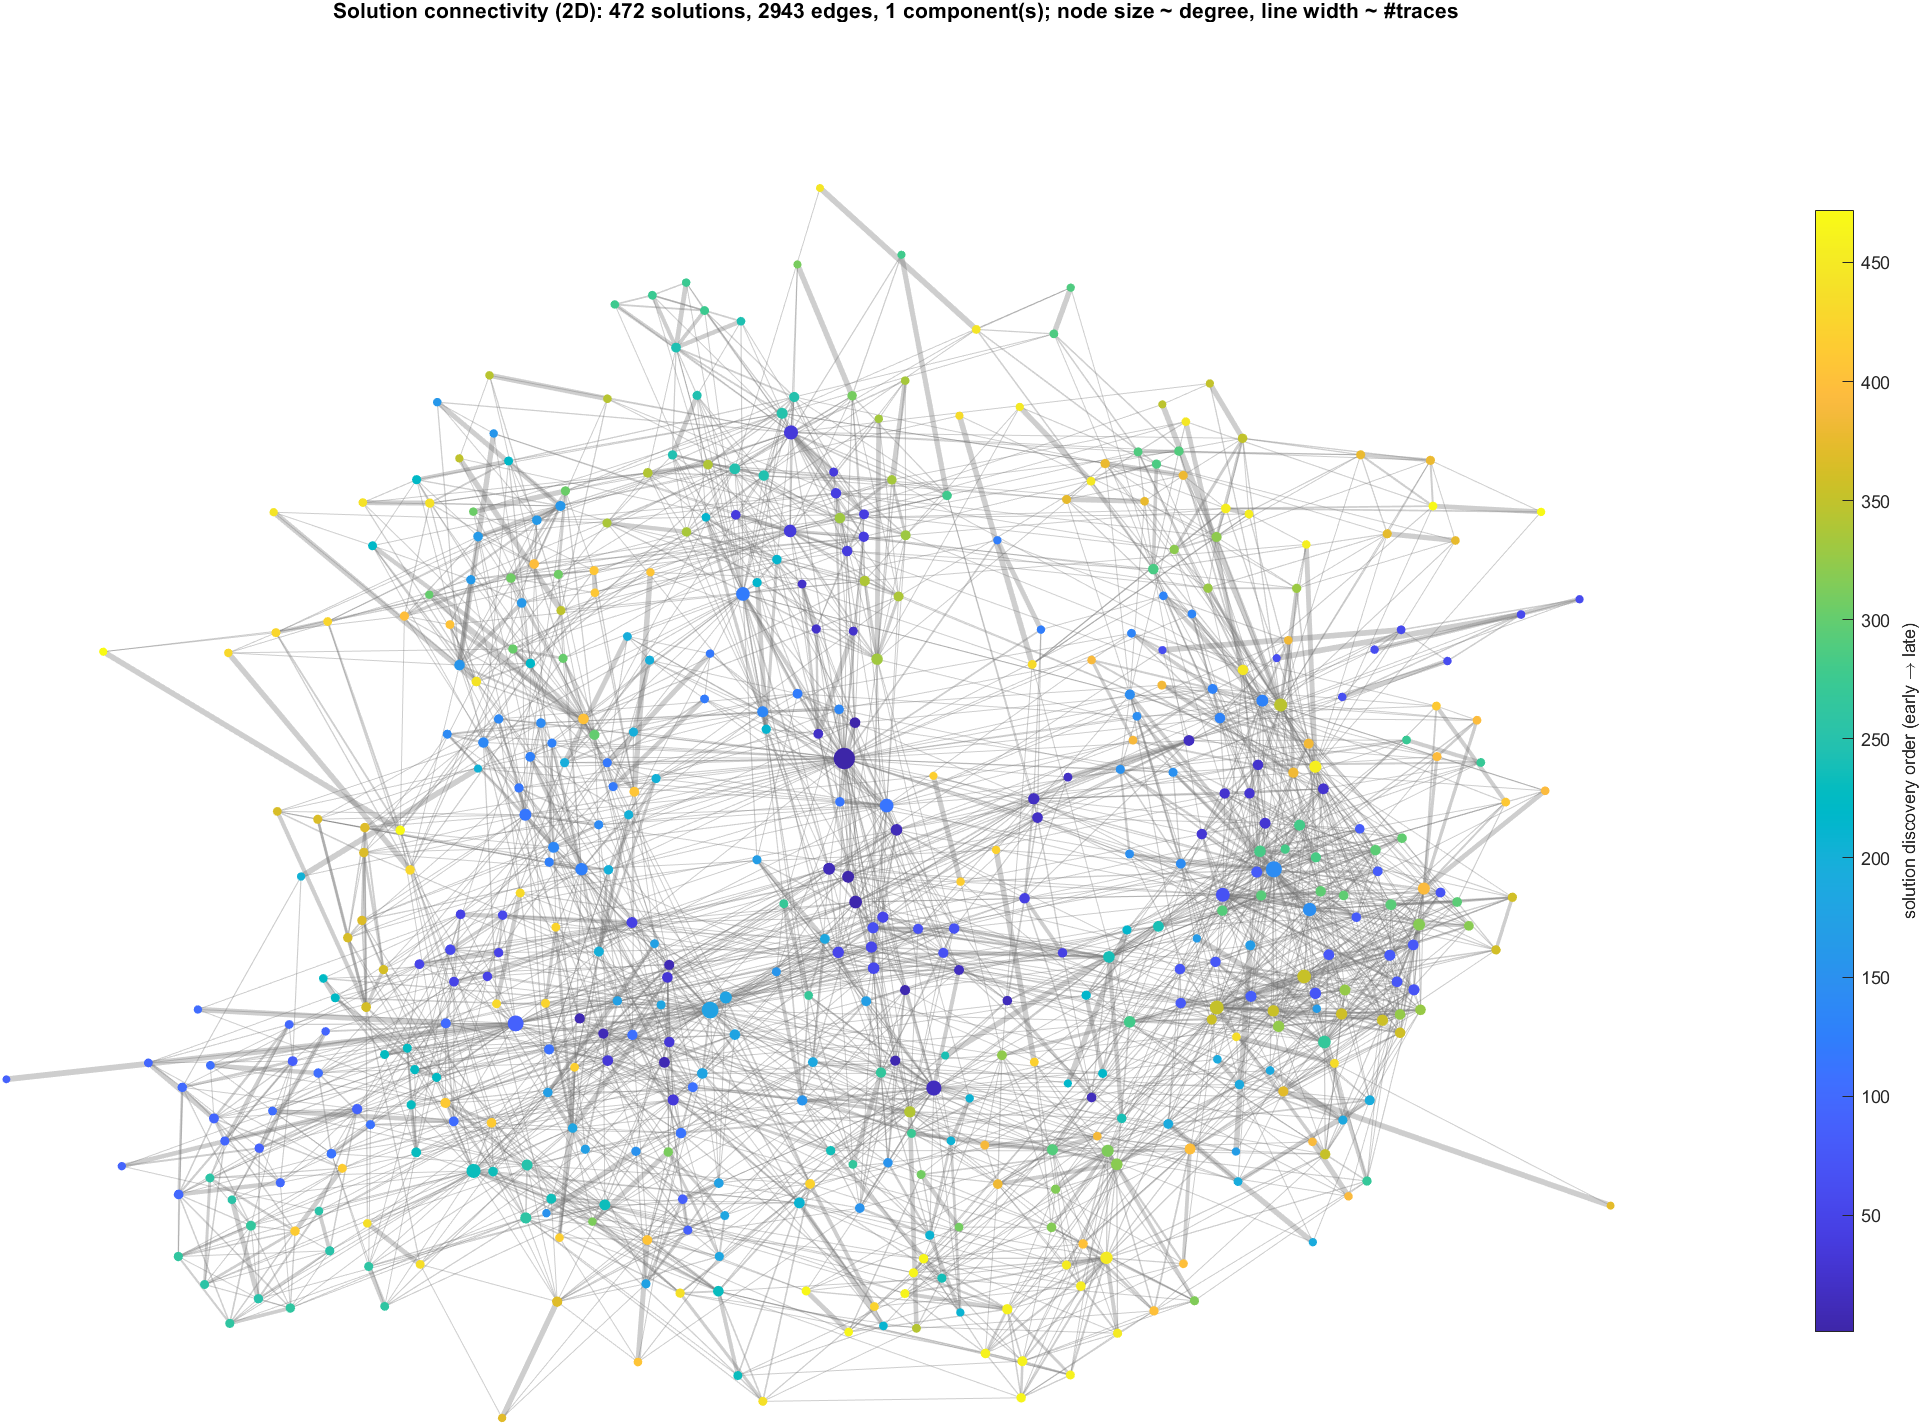
\includegraphics[width=0.96\textwidth]{connectivity_case30_v4_reference.png}
\caption{case30 released-v4 reference connectivity: 472 solutions, 2,943
unique edges, and one connected component. Node color records reference-run
discovery order; node size is degree and line width counts shared traces. The
solution-set distance to the saved v5 reference is $9.45\times10^{-12}$.}
\end{figure}}{}
\IfFileExists{connectivity_case57_v4_reference.png}{
\begin{figure}[p]\centering
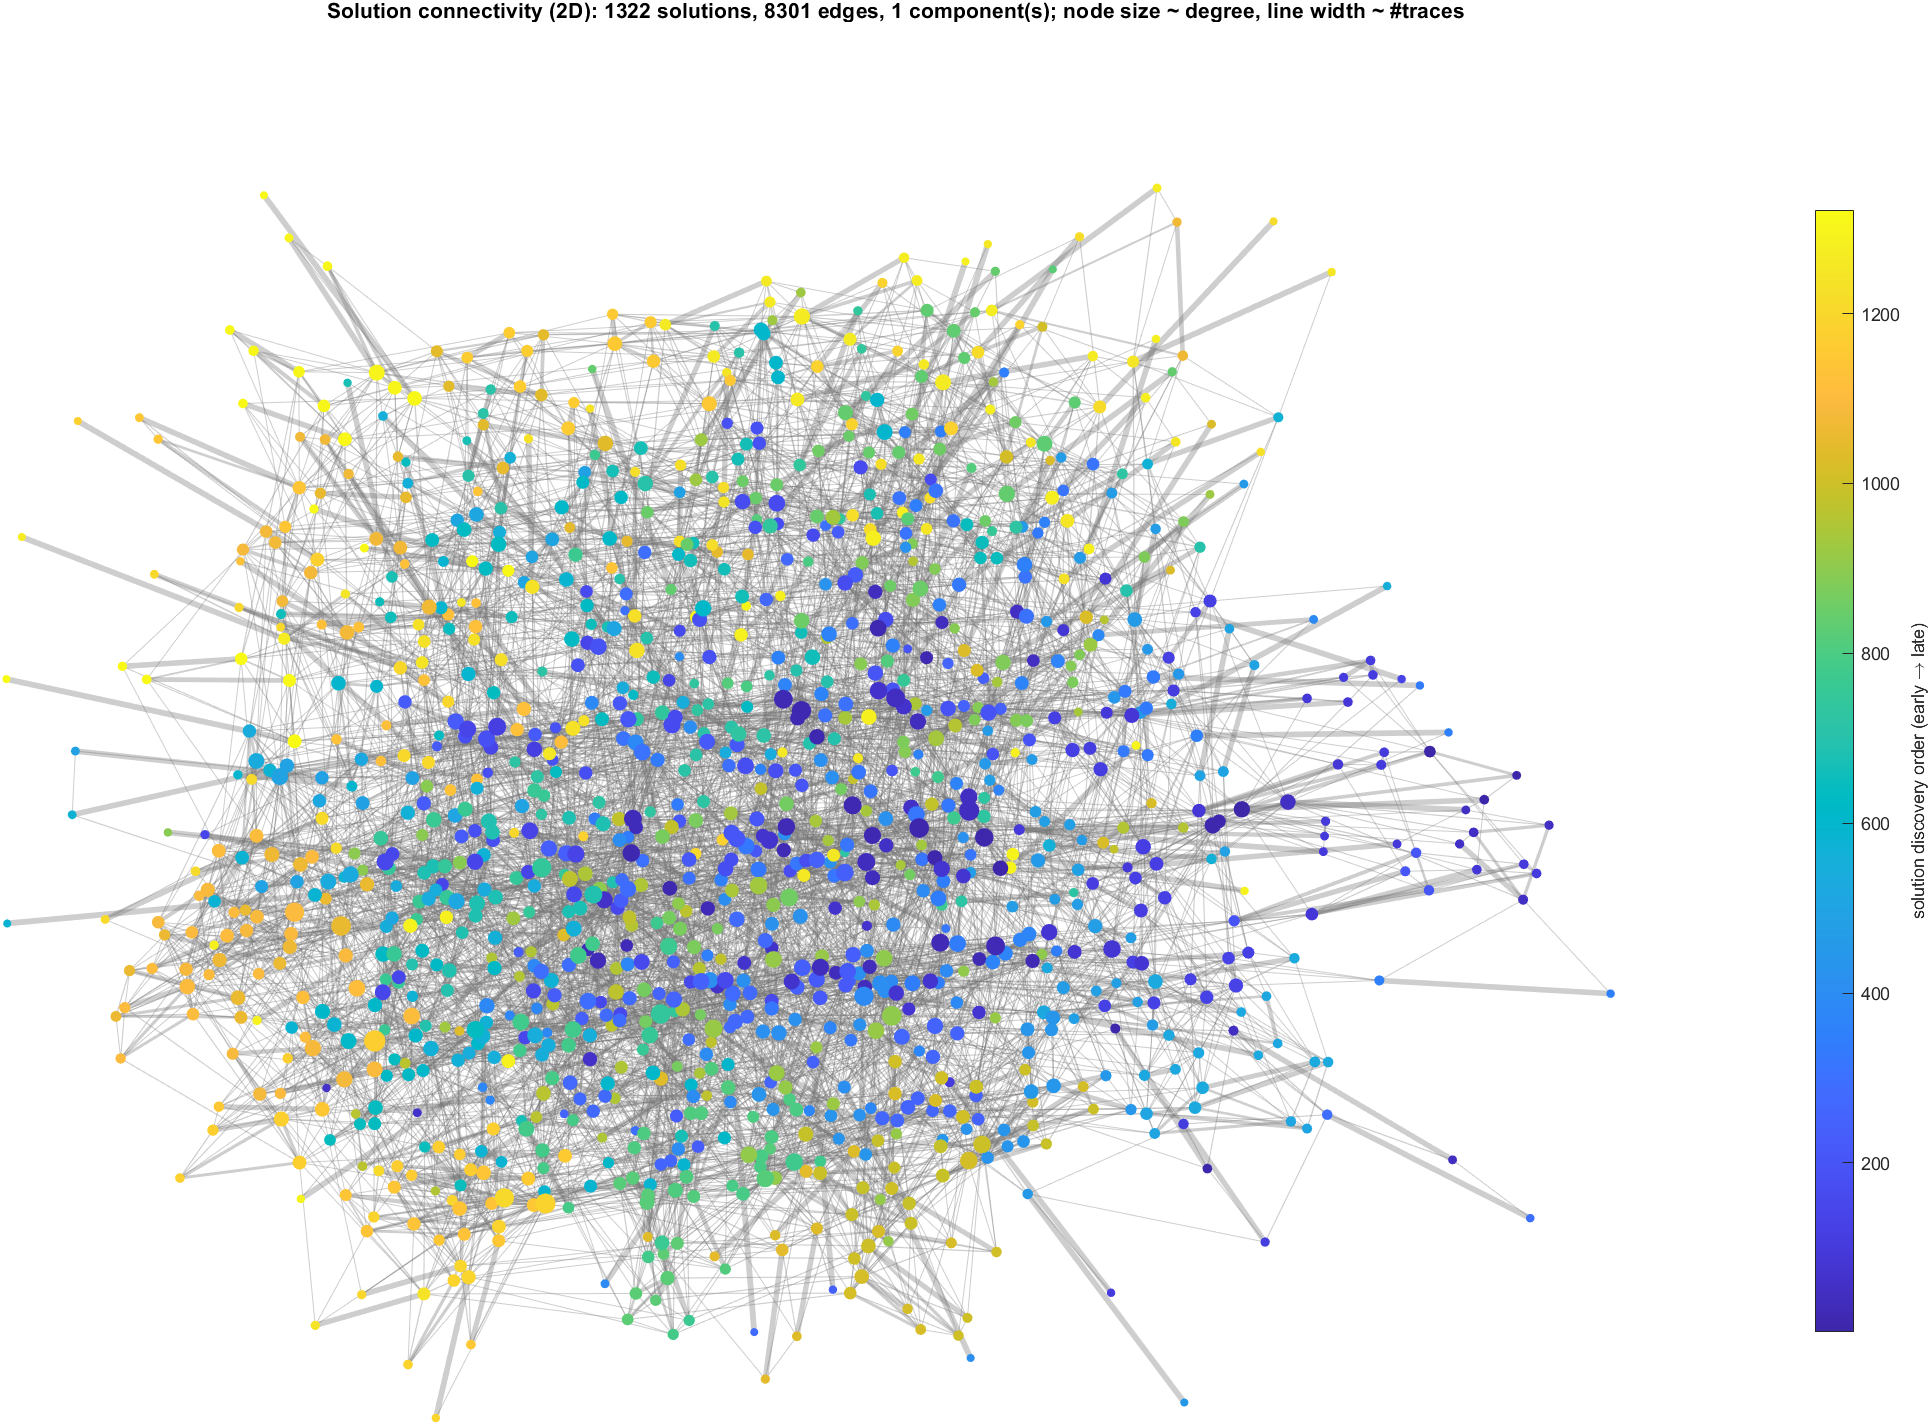
\includegraphics[width=0.96\textwidth]{connectivity_case57_v4_reference.png}
\caption{case57 released-v4 reference connectivity: 1,322 solutions, 8,301
unique edges, and one connected component. Node color records reference-run
discovery order; node size is degree and line width counts shared traces. The
solution-set distance to the saved v5 reference is $2.00\times10^{-10}$.}
\end{figure}}{}

All 180 timing runs returned expected counts. Independent symmetric nearest-set
validation passed 40/40 comparisons; worst distance was
$2.6591\times10^{-9}$ against a $4\times10^{-7}$ tolerance. The bundled
\code{test_checkpoint_policy_compatibility_v5.m} and \code{smoke_test_v5.m}
remain available for platform-specific checks, but results from non-designated
machines are not published. The full report and per-case table are in
\code{SCHEDULER_BENCHMARK_v5.md} and the published CSV files.

\section{Direct released-v4 performance baseline}
The retained v4 pass used the same 20 cases, MATLAB R2022a, Windows x64, and 23
workers. MEX v4 required 718.656~s and pure MATLAB v4 1272.966~s, both returning
3256 total solutions. V5 scan averaged 606.947~s, descriptively 15.5\% below
the historical MEX value. Because v4 is one retained pass and v5 is a current
three-repeat experiment, this is release context rather than a controlled paired
speedup claim.
